% Seminarul 6: Modele VAR și cauzalitate Granger
% Serii de timp -- Programele de licență Informatică economică și Cibernetică economică, Academia de Studii Economice din București
% GENERAT de latex/build_seminar6.py -- modificați generatorul, nu acest fișier.
% Implicit versiunea pentru studenți; versiunea profesorului este wrapper-ul *_solutions.tex.
\makeatletter\@ifundefined{ifsolutions}{\expandafter\newif\csname ifsolutions\endcsname}{}\makeatother

\newcommand{\coursename}{Serii de timp}
\def\tsalang{ro}
% Preambul comun TSA -- Serii de timp / Time Series Analysis (Beamer, 16:9)
% Același design ca MFM și SFM (preluat din SFM, 5 octombrie 2026). Înainte de % Preambul comun TSA -- Serii de timp / Time Series Analysis (Beamer, 16:9)
% Același design ca MFM și SFM (preluat din SFM, 5 octombrie 2026). Înainte de % Preambul comun TSA -- Serii de timp / Time Series Analysis (Beamer, 16:9)
% Același design ca MFM și SFM (preluat din SFM, 5 octombrie 2026). Înainte de \input{../../latex/preamble} se definește
%   \newcommand{\coursename}{Time Series Analysis}      (EN)
%   \newcommand{\coursename}{Serii de timp}       (RO)  și  \def\tsalang{ro}
% Fișierele .tex se află în EN/Courses, EN/Seminars, RO/Cursuri, RO/Seminarii (două niveluri sub rădăcină).
% Deck-urile sînt generate de latex/build_chapterN.py / build_seminarN.py (vezi latex/tsa_build.py).

\documentclass[9pt, aspectratio=169, t]{beamer}
\providecommand{\coursename}{Time Series Analysis}

% Ensure content fits on slides
\setbeamersize{text margin left=8mm, text margin right=8mm}
% Smaller institute font (title page)
\setbeamerfont{institute}{size=\footnotesize}

%=============================================================================
% THEME AND STYLE CONFIGURATION
%=============================================================================
\usetheme{default}
% Using default theme for clean header/footer control

% Color Palette (matching Redispatch PDF)
\definecolor{MainBlue}{RGB}{26, 58, 110}
\definecolor{AccentBlue}{RGB}{26, 58, 110}
\definecolor{IDAred}{RGB}{205, 0, 0}
\definecolor{DarkGray}{RGB}{51, 51, 51}
\definecolor{MediumGray}{RGB}{128, 128, 128}
\definecolor{LightGray}{RGB}{248, 248, 248}
\definecolor{VeryLightGray}{RGB}{235, 235, 235}
\definecolor{KeynoteGray}{RGB}{218, 218, 218}
\definecolor{SectionGray}{RGB}{120, 120, 120}
\definecolor{FooterGray}{RGB}{100, 100, 100}
\definecolor{Crimson}{RGB}{220, 53, 69}
\definecolor{Forest}{RGB}{46, 125, 50}
\definecolor{Amber}{RGB}{181, 133, 63}
\definecolor{Orange}{RGB}{230, 126, 34}
\definecolor{Purple}{RGB}{142, 68, 173}

% Gradient background (exact Keynote 315° gradient: white to RGB 218,218,218)
\setbeamertemplate{background}{%
    \begin{tikzpicture}[remember picture, overlay]
        \shade[shading=axis, shading angle=315,
        top color=white, bottom color=KeynoteGray]
        (current page.south west) rectangle (current page.north east);
    \end{tikzpicture}%
}
% Fallback solid color for compatibility
\setbeamercolor{background canvas}{bg=}

\setbeamercolor{palette primary}{bg=MainBlue, fg=white}
\setbeamercolor{palette secondary}{bg=MainBlue!85, fg=white}
\setbeamercolor{palette tertiary}{bg=MainBlue!70, fg=white}
\setbeamercolor{structure}{fg=MainBlue}
\setbeamercolor{title}{fg=IDAred}
\setbeamercolor{frametitle}{fg=IDAred, bg=}
\setbeamercolor{block title}{bg=MainBlue, fg=white}
\setbeamercolor{block body}{bg=VeryLightGray, fg=DarkGray}
\setbeamercolor{block title alerted}{bg=Crimson, fg=white}
\setbeamercolor{block body alerted}{bg=Crimson!8, fg=DarkGray}
\setbeamercolor{block title example}{bg=Forest, fg=white}
\setbeamercolor{block body example}{bg=Forest!8, fg=DarkGray}
\setbeamercolor{item}{fg=MainBlue}

% Footer colors (override Madrid theme blue)
\setbeamercolor{author in head/foot}{fg=FooterGray, bg=}
\setbeamercolor{title in head/foot}{fg=FooterGray, bg=}
\setbeamercolor{date in head/foot}{fg=FooterGray, bg=}
\setbeamercolor{section in head/foot}{fg=FooterGray, bg=}
\setbeamercolor{subsection in head/foot}{fg=FooterGray, bg=}

% Bullet styles (apply everywhere including blocks)
\setbeamertemplate{itemize item}{\color{MainBlue}$\boxdot$}
\setbeamertemplate{itemize subitem}{\color{MainBlue}$\blacktriangleright$}
\setbeamertemplate{itemize subsubitem}{\color{MainBlue}\tiny$\bullet$}
\setbeamertemplate{itemize/enumerate body begin}{\normalsize}
\setbeamertemplate{itemize/enumerate subbody begin}{\normalsize}

% Item spacing - compact style
\setlength{\leftmargini}{10pt}       % Level 1: minimal indent
\setlength{\leftmarginii}{10pt}      % Level 2: minimal additional indent
% Compact list spacing (zero extra space before/after lists in blocks)
\makeatletter
\def\@listi{\leftmargin\leftmargini \topsep 0pt \parsep 0pt \itemsep 0pt}
\def\@listii{\leftmargin\leftmarginii \topsep 0pt \parsep 0pt \itemsep 0pt}
\makeatother

\setbeamertemplate{navigation symbols}{}

%=============================================================================
% CUSTOM HEADLINE
%=============================================================================
\setbeamertemplate{headline}{%
    \vskip10pt%
    \hbox to \paperwidth{%
        \hskip0.5cm%
        {\small\color{FooterGray}\renewcommand{\hyperlink}[2]{##2}\insertsectionhead}%
        \hfill%
        \textcolor{FooterGray}{\small\insertframenumber}%
        \hskip0.5cm%
    }%
    \vskip4pt%
    {\color{FooterGray}\hrule height 0.4pt}%
}

%=============================================================================
% CUSTOM FOOTER
%=============================================================================
\usepackage{fontawesome5}

\setbeamertemplate{footline}{%
    {\color{FooterGray}\hrule height 0.4pt}%
    \vskip4pt%
    \hbox to \paperwidth{%
        \hskip0.5cm%
        \textcolor{FooterGray}{\small\coursename}%
        \hfill%
        \raisebox{-0.1em}{%
            \begin{tikzpicture}[x=0.08em, y=0.08em, line width=0.4pt]
                \draw[FooterGray] (0,3) -- (1,4) -- (2,3.5) -- (3,5) -- (4,4) -- (5,6) -- (6,5.5) -- (7,4) -- (8,5) -- (9,7) -- (10,6) -- (11,5) -- (12,6.5) -- (13,8) -- (14,7) -- (15,6) -- (16,7.5) -- (17,9) -- (18,8) -- (19,7) -- (20,8.5) -- (21,10) -- (22,9) -- (23,8) -- (24,9.5);
            \end{tikzpicture}%
        }%
        \hskip0.5cm%
    }%
    \vskip6pt%
}

%=============================================================================
% PACKAGES
%=============================================================================
\usepackage[utf8]{inputenc}
\DeclareUnicodeCharacter{03B1}{\ensuremath{\alpha}}
\usepackage[T1]{fontenc}
\usepackage{amsmath, amssymb, amsthm}
\usepackage{mathtools}
\usepackage{bm}
\usepackage{tikz}
\usetikzlibrary{arrows.meta, positioning, shapes, calc, decorations.pathreplacing, shadings}
\usepackage{booktabs}
\usepackage{multirow}
\usepackage{array}
\usepackage{graphicx}
\usepackage{animate}
\usepackage{hyperref}
\usepackage{colortbl}
\usepackage{listings}
\lstset{language=Python, basicstyle=\ttfamily\scriptsize, keywordstyle=\color{MainBlue}\bfseries,
  commentstyle=\color{Forest}, stringstyle=\color{Crimson}, breaklines=true,
  frame=none, backgroundcolor=\color{VeryLightGray}, xleftmargin=2mm}
\hypersetup{colorlinks=true, linkcolor=MainBlue, urlcolor=MainBlue}
\graphicspath{{../../logos/}{../../charts/}{../../photos/}}
\usepackage{xcolor}
\hfuzz=2pt  % Suppress tiny overfull warnings (<2pt)
\vfuzz=2pt  % Suppress tiny vertical overfull warnings (<2pt)
% \mathrm in the sans-serif family of the slides (beamer resets \mathrm to the serif family at \begin{document};
% this hook runs after beamer's, so WN, Var, RMSE, ... in formulas match the surrounding text)
% Bold vectors and matrices in the same sans-serif family: \mathbf{A} in sans bold (beamer's own \mathbf came out in
% medium weight), and the bold upright Greek capitals of \boldsymbol / \bm (\bSigma, \bPhi, \boldsymbol{\Theta}) in
% cmss bold: bm.sty fixes its "boldoperators" font when it is loaded (serif cmbx), before beamer switches the
% operators to cmss, so it is reset here.
\AtBeginDocument{%
  \SetMathAlphabet{\mathrm}{normal}{\encodingdefault}{\sfdefault}{\mddefault}{n}%
  \SetMathAlphabet{\mathrm}{bold}{\encodingdefault}{\sfdefault}{bx}{n}%
  \SetMathAlphabet{\mathbf}{normal}{\encodingdefault}{\sfdefault}{bx}{n}%
  \SetMathAlphabet{\mathbf}{bold}{\encodingdefault}{\sfdefault}{bx}{n}%
  \SetSymbolFont{boldoperators}{normal}{OT1}{cmss}{bx}{n}%
  \SetSymbolFont{boldoperators}{bold}{OT1}{cmss}{bx}{n}}

%=============================================================================
% QUANTLET COMMANDS
%   \quantlet{<displayed name>}{<url>}       (generic, compatible with the older TSA decks)
%   \tsaquantlet{Ch_05}{TSA_ch5_garch}       -> https://github.com/danpele/Time-Series-Analysis/tree/main/Quantlets/Ch_05/TSA_ch5_garch
%   \qlurl{<folder>} is defined per chapter by the generator (Quantlets/Ch_NN/<folder>)
%=============================================================================
\newcommand{\tsarepo}{https://github.com/danpele/Time-Series-Analysis}
\newcommand{\tsaqlbase}{https://github.com/danpele/Time-Series-Analysis/tree/main/Quantlets}
\newcommand{\quantlet}[2]{%
    \hfill\href{#2}{%
        \raisebox{-0.15em}{
\includegraphics[height=0.7em]{ql_logo.png}}%
        \textcolor{MainBlue}{\tiny\ #1}%
    }%
}
\newcommand{\tsaquantlet}[2]{\quantlet{\detokenize{#2}}{\tsaqlbase/#1/#2}}

%=============================================================================
% NOTEBOOKS (Google Colab)
%   \colaburl{notebooks/EN/chapter5_seminar_notebook.ipynb} -> the Colab link of a file in the TSA repo
%   \nb: the chapter notebook (each seminar deck redefines it with \renewcommand)
%=============================================================================
\newcommand{\colaburl}[1]{https://colab.research.google.com/github/danpele/Time-Series-Analysis/blob/main/#1}
\newcommand{\nb}{https://colab.research.google.com/github/danpele/Time-Series-Analysis/tree/main/notebooks/EN}
\newcommand{\nbname}{notebooks/EN}

%=============================================================================
% SLIDE HELPERS (used by the generators; the same as in MFM)
%=============================================================================
% local font size for list bodies (the preamble forces \normalsize)
\newcommand{\itemsize}[1]{\setbeamertemplate{itemize/enumerate body begin}{#1}\setbeamertemplate{itemize/enumerate subbody begin}{#1}}
\newcommand{\intitle}[1]{{\hypersetup{urlcolor=white}#1}}   % white links inside coloured title bars
\newcommand{\imgcap}[1]{{\scriptsize #1}\\[0.5mm]}          % caption under a photo
\newcommand{\imgcredit}[2]{{\tiny\color{FooterGray}\href{#1}{#2}}}   % image credit: source URL, author/licence
\newcommand{\aiprompt}[1]{{\ttfamily\color{MainBlue}#1}}     % a prompt to an AI assistant

%=============================================================================
% SEMINARS: student version by default; the instructor wrapper *_solutions.tex sets \solutionstrue
%=============================================================================
\makeatletter\@ifundefined{ifsolutions}{\expandafter\newif\csname ifsolutions\endcsname}{}\makeatother
\newcommand{\solonly}[1]{\ifsolutions #1\fi}
\newcommand{\propsub}{\ifsolutions\else\framesubtitle{\ifdefined\tsalang Rezolvarea se discută la seminar\else Solution discussed in class\fi}\fi}

%=============================================================================
% APPENDIX AND CHAPTER LINKS (latex/appendix_links.py writes the calls; it also re-declares these
% macros before \begin{document}, so the decks compile with or without this preamble block)
%=============================================================================
\providecommand{\tsaapplink}[3]{\hypertarget{#2}{}\hyperlink{#1}{\beamergotobutton{#3}}}
\providecommand{\tsaappback}[2]{\begin{tikzpicture}[remember picture,overlay]\node[anchor=south east] at ([xshift=-3mm,yshift=7mm]current page.south east){\hyperlink{#1}{\beamerreturnbutton{#2}}};\end{tikzpicture}}
\providecommand{\tsachlink}[2]{\href{#1}{#2}}
\providecommand{\tsachlinkt}[2]{\href{#1}{\usebeamercolor[fg]{frametitle}#2}}

%=============================================================================
% QUANTINAR COMMAND: link către un curs Quantinar (subiecte avansate)
%=============================================================================
\newcommand{\quantinar}[2]{%
    \href{#2}{%
        \raisebox{-0.15em}{
\includegraphics[height=0.8em]{qr_logo.png}}%
        \textcolor{MainBlue}{\scriptsize\ #1}%
    }%
}

%=============================================================================
% CUSTOM TITLE PAGE
%=============================================================================
\defbeamertemplate*{title page}{hybrid}[1][]
{
    \vspace{0.2cm}
    % Logos row - top header (with clickable links)
    \begin{center}
        \href{https://www.ase.ro}{
\includegraphics[height=1.0cm]{ase_logo.png}}\hspace{0.3cm}%
        \href{https://theida.net}{
\includegraphics[height=1.0cm]{ida_logo.png}}\hspace{0.3cm}%
        \href{https://blockchain-research-center.com}{
\includegraphics[height=1.0cm]{brc_logo.png}}\hspace{0.3cm}%
        \href{https://www.ai4efin.ase.ro}{
\includegraphics[height=1.0cm]{ai4efin_logo.png}}\hspace{0.3cm}%
        \href{https://ipe.ro/new}{
\includegraphics[height=1.0cm]{acad_logo.png}}\hspace{0.3cm}%
        \href{https://www.digital-finance-msca.com}{
\includegraphics[height=1.0cm]{msca_logo.png}}%
    \end{center}

    \vspace{0.6cm}

    % Main title with Q logos on sides (with clickable links)
    \begin{center}
        \begin{minipage}{0.1\textwidth}
            \centering
            \href{https://quantlet.com}{
\includegraphics[height=1.1cm]{ql_logo.png}}
        \end{minipage}%
        \begin{minipage}{0.78\textwidth}
            \centering
            {\LARGE\bfseries\usebeamercolor[fg]{title}\inserttitle}

            \vspace{0.3cm}

            {\usebeamerfont{subtitle}\usebeamercolor[fg]{title}\insertsubtitle}
        \end{minipage}%
        \begin{minipage}{0.1\textwidth}
            \centering
            \href{https://quantinar.com}{
\includegraphics[height=1.1cm]{qr_logo.png}}
        \end{minipage}
    \end{center}

    \vspace{0.6cm}

    % Authors (left aligned)
    \hspace{0.5cm}{\usebeamerfont{author}\insertauthor}

    \vspace{0.3cm}

    % Institute/Affiliations (left aligned)
    \hspace{0.5cm}\begin{minipage}[t]{0.9\textwidth}
        \raggedright\small\insertinstitute
    \end{minipage}
}

%=============================================================================
% THEOREM ENVIRONMENTS
%=============================================================================
\theoremstyle{definition}
\setbeamertemplate{theorems}[numbered]
\ifdefined\tsalang
\newtheorem{defn}{Definiție}
\newtheorem{thm}{Teoremă}
\newtheorem{prop}{Propoziție}
\newtheorem{rmk}{Observație}
\else
\newtheorem{defn}{Definition}
\newtheorem{thm}{Theorem}
\newtheorem{prop}{Proposition}
\newtheorem{rmk}{Remark}
\fi

%=============================================================================
% CENTRED MINIPAGE (no extra vertical space)
%=============================================================================
\newenvironment{cminipage}[1]{%
    \par\noindent\hfill\begin{minipage}{#1}\ignorespaces
}{%
    \end{minipage}\hfill\null\par
}

%=============================================================================
% CUSTOM COMMANDS
%=============================================================================
\newcommand{\E}{\mathbb{E}}
\newcommand{\Var}{\text{Var}}
\newcommand{\Cov}{\text{Cov}}
\newcommand{\Corr}{\text{Corr}}
\newcommand{\R}{\mathbb{R}}
\newcommand{\N}{\mathbb{N}}
\newcommand{\Z}{\mathbb{Z}}
\newcommand{\B}{\mathbf{B}}
\newcommand{\imark}{\textcolor{MainBlue}{\textbullet}}
\newcommand{\RMSE}{\text{RMSE}}
\newcommand{\MAE}{\text{MAE}}
\newcommand{\MAPE}{\text{MAPE}}

% Boldface vector/matrix commands (VAR, VECM, state space; also used by the older TSA decks)
\newcommand{\bY}{\mathbf{Y}}
\newcommand{\bX}{\mathbf{X}}
\newcommand{\bA}{\mathbf{A}}
\newcommand{\bB}{\mathbf{B}}
\newcommand{\bepsilon}{\boldsymbol{\varepsilon}}
\newcommand{\bSigma}{\boldsymbol{\Sigma}}
\newcommand{\bPhi}{\boldsymbol{\Phi}}
\newcommand{\bGamma}{\boldsymbol{\Gamma}}
\newcommand{\bPi}{\boldsymbol{\Pi}}
\newcommand{\bc}{\mathbf{c}}
\newcommand{\balpha}{\boldsymbol{\alpha}}
\newcommand{\bbeta}{\boldsymbol{\beta}}
\newcommand{\bvarepsilon}{\boldsymbol{\varepsilon}}

% Legacy seminar marks (older TSA seminar decks)
\newcommand{\correct}{\textcolor{Forest}{\checkmark}}
\newcommand{\incorrect}{\textcolor{Crimson}{\texttimes}}
 se definește
%   \newcommand{\coursename}{Time Series Analysis}      (EN)
%   \newcommand{\coursename}{Serii de timp}       (RO)  și  \def\tsalang{ro}
% Fișierele .tex se află în EN/Courses, EN/Seminars, RO/Cursuri, RO/Seminarii (două niveluri sub rădăcină).
% Deck-urile sînt generate de latex/build_chapterN.py / build_seminarN.py (vezi latex/tsa_build.py).

\documentclass[9pt, aspectratio=169, t]{beamer}
\providecommand{\coursename}{Time Series Analysis}

% Ensure content fits on slides
\setbeamersize{text margin left=8mm, text margin right=8mm}
% Smaller institute font (title page)
\setbeamerfont{institute}{size=\footnotesize}

%=============================================================================
% THEME AND STYLE CONFIGURATION
%=============================================================================
\usetheme{default}
% Using default theme for clean header/footer control

% Color Palette (matching Redispatch PDF)
\definecolor{MainBlue}{RGB}{26, 58, 110}
\definecolor{AccentBlue}{RGB}{26, 58, 110}
\definecolor{IDAred}{RGB}{205, 0, 0}
\definecolor{DarkGray}{RGB}{51, 51, 51}
\definecolor{MediumGray}{RGB}{128, 128, 128}
\definecolor{LightGray}{RGB}{248, 248, 248}
\definecolor{VeryLightGray}{RGB}{235, 235, 235}
\definecolor{KeynoteGray}{RGB}{218, 218, 218}
\definecolor{SectionGray}{RGB}{120, 120, 120}
\definecolor{FooterGray}{RGB}{100, 100, 100}
\definecolor{Crimson}{RGB}{220, 53, 69}
\definecolor{Forest}{RGB}{46, 125, 50}
\definecolor{Amber}{RGB}{181, 133, 63}
\definecolor{Orange}{RGB}{230, 126, 34}
\definecolor{Purple}{RGB}{142, 68, 173}

% Gradient background (exact Keynote 315° gradient: white to RGB 218,218,218)
\setbeamertemplate{background}{%
    \begin{tikzpicture}[remember picture, overlay]
        \shade[shading=axis, shading angle=315,
        top color=white, bottom color=KeynoteGray]
        (current page.south west) rectangle (current page.north east);
    \end{tikzpicture}%
}
% Fallback solid color for compatibility
\setbeamercolor{background canvas}{bg=}

\setbeamercolor{palette primary}{bg=MainBlue, fg=white}
\setbeamercolor{palette secondary}{bg=MainBlue!85, fg=white}
\setbeamercolor{palette tertiary}{bg=MainBlue!70, fg=white}
\setbeamercolor{structure}{fg=MainBlue}
\setbeamercolor{title}{fg=IDAred}
\setbeamercolor{frametitle}{fg=IDAred, bg=}
\setbeamercolor{block title}{bg=MainBlue, fg=white}
\setbeamercolor{block body}{bg=VeryLightGray, fg=DarkGray}
\setbeamercolor{block title alerted}{bg=Crimson, fg=white}
\setbeamercolor{block body alerted}{bg=Crimson!8, fg=DarkGray}
\setbeamercolor{block title example}{bg=Forest, fg=white}
\setbeamercolor{block body example}{bg=Forest!8, fg=DarkGray}
\setbeamercolor{item}{fg=MainBlue}

% Footer colors (override Madrid theme blue)
\setbeamercolor{author in head/foot}{fg=FooterGray, bg=}
\setbeamercolor{title in head/foot}{fg=FooterGray, bg=}
\setbeamercolor{date in head/foot}{fg=FooterGray, bg=}
\setbeamercolor{section in head/foot}{fg=FooterGray, bg=}
\setbeamercolor{subsection in head/foot}{fg=FooterGray, bg=}

% Bullet styles (apply everywhere including blocks)
\setbeamertemplate{itemize item}{\color{MainBlue}$\boxdot$}
\setbeamertemplate{itemize subitem}{\color{MainBlue}$\blacktriangleright$}
\setbeamertemplate{itemize subsubitem}{\color{MainBlue}\tiny$\bullet$}
\setbeamertemplate{itemize/enumerate body begin}{\normalsize}
\setbeamertemplate{itemize/enumerate subbody begin}{\normalsize}

% Item spacing - compact style
\setlength{\leftmargini}{10pt}       % Level 1: minimal indent
\setlength{\leftmarginii}{10pt}      % Level 2: minimal additional indent
% Compact list spacing (zero extra space before/after lists in blocks)
\makeatletter
\def\@listi{\leftmargin\leftmargini \topsep 0pt \parsep 0pt \itemsep 0pt}
\def\@listii{\leftmargin\leftmarginii \topsep 0pt \parsep 0pt \itemsep 0pt}
\makeatother

\setbeamertemplate{navigation symbols}{}

%=============================================================================
% CUSTOM HEADLINE
%=============================================================================
\setbeamertemplate{headline}{%
    \vskip10pt%
    \hbox to \paperwidth{%
        \hskip0.5cm%
        {\small\color{FooterGray}\renewcommand{\hyperlink}[2]{##2}\insertsectionhead}%
        \hfill%
        \textcolor{FooterGray}{\small\insertframenumber}%
        \hskip0.5cm%
    }%
    \vskip4pt%
    {\color{FooterGray}\hrule height 0.4pt}%
}

%=============================================================================
% CUSTOM FOOTER
%=============================================================================
\usepackage{fontawesome5}

\setbeamertemplate{footline}{%
    {\color{FooterGray}\hrule height 0.4pt}%
    \vskip4pt%
    \hbox to \paperwidth{%
        \hskip0.5cm%
        \textcolor{FooterGray}{\small\coursename}%
        \hfill%
        \raisebox{-0.1em}{%
            \begin{tikzpicture}[x=0.08em, y=0.08em, line width=0.4pt]
                \draw[FooterGray] (0,3) -- (1,4) -- (2,3.5) -- (3,5) -- (4,4) -- (5,6) -- (6,5.5) -- (7,4) -- (8,5) -- (9,7) -- (10,6) -- (11,5) -- (12,6.5) -- (13,8) -- (14,7) -- (15,6) -- (16,7.5) -- (17,9) -- (18,8) -- (19,7) -- (20,8.5) -- (21,10) -- (22,9) -- (23,8) -- (24,9.5);
            \end{tikzpicture}%
        }%
        \hskip0.5cm%
    }%
    \vskip6pt%
}

%=============================================================================
% PACKAGES
%=============================================================================
\usepackage[utf8]{inputenc}
\DeclareUnicodeCharacter{03B1}{\ensuremath{\alpha}}
\usepackage[T1]{fontenc}
\usepackage{amsmath, amssymb, amsthm}
\usepackage{mathtools}
\usepackage{bm}
\usepackage{tikz}
\usetikzlibrary{arrows.meta, positioning, shapes, calc, decorations.pathreplacing, shadings}
\usepackage{booktabs}
\usepackage{multirow}
\usepackage{array}
\usepackage{graphicx}
\usepackage{animate}
\usepackage{hyperref}
\usepackage{colortbl}
\usepackage{listings}
\lstset{language=Python, basicstyle=\ttfamily\scriptsize, keywordstyle=\color{MainBlue}\bfseries,
  commentstyle=\color{Forest}, stringstyle=\color{Crimson}, breaklines=true,
  frame=none, backgroundcolor=\color{VeryLightGray}, xleftmargin=2mm}
\hypersetup{colorlinks=true, linkcolor=MainBlue, urlcolor=MainBlue}
\graphicspath{{../../logos/}{../../charts/}{../../photos/}}
\usepackage{xcolor}
\hfuzz=2pt  % Suppress tiny overfull warnings (<2pt)
\vfuzz=2pt  % Suppress tiny vertical overfull warnings (<2pt)
% \mathrm in the sans-serif family of the slides (beamer resets \mathrm to the serif family at \begin{document};
% this hook runs after beamer's, so WN, Var, RMSE, ... in formulas match the surrounding text)
% Bold vectors and matrices in the same sans-serif family: \mathbf{A} in sans bold (beamer's own \mathbf came out in
% medium weight), and the bold upright Greek capitals of \boldsymbol / \bm (\bSigma, \bPhi, \boldsymbol{\Theta}) in
% cmss bold: bm.sty fixes its "boldoperators" font when it is loaded (serif cmbx), before beamer switches the
% operators to cmss, so it is reset here.
\AtBeginDocument{%
  \SetMathAlphabet{\mathrm}{normal}{\encodingdefault}{\sfdefault}{\mddefault}{n}%
  \SetMathAlphabet{\mathrm}{bold}{\encodingdefault}{\sfdefault}{bx}{n}%
  \SetMathAlphabet{\mathbf}{normal}{\encodingdefault}{\sfdefault}{bx}{n}%
  \SetMathAlphabet{\mathbf}{bold}{\encodingdefault}{\sfdefault}{bx}{n}%
  \SetSymbolFont{boldoperators}{normal}{OT1}{cmss}{bx}{n}%
  \SetSymbolFont{boldoperators}{bold}{OT1}{cmss}{bx}{n}}

%=============================================================================
% QUANTLET COMMANDS
%   \quantlet{<displayed name>}{<url>}       (generic, compatible with the older TSA decks)
%   \tsaquantlet{Ch_05}{TSA_ch5_garch}       -> https://github.com/danpele/Time-Series-Analysis/tree/main/Quantlets/Ch_05/TSA_ch5_garch
%   \qlurl{<folder>} is defined per chapter by the generator (Quantlets/Ch_NN/<folder>)
%=============================================================================
\newcommand{\tsarepo}{https://github.com/danpele/Time-Series-Analysis}
\newcommand{\tsaqlbase}{https://github.com/danpele/Time-Series-Analysis/tree/main/Quantlets}
\newcommand{\quantlet}[2]{%
    \hfill\href{#2}{%
        \raisebox{-0.15em}{
\includegraphics[height=0.7em]{ql_logo.png}}%
        \textcolor{MainBlue}{\tiny\ #1}%
    }%
}
\newcommand{\tsaquantlet}[2]{\quantlet{\detokenize{#2}}{\tsaqlbase/#1/#2}}

%=============================================================================
% NOTEBOOKS (Google Colab)
%   \colaburl{notebooks/EN/chapter5_seminar_notebook.ipynb} -> the Colab link of a file in the TSA repo
%   \nb: the chapter notebook (each seminar deck redefines it with \renewcommand)
%=============================================================================
\newcommand{\colaburl}[1]{https://colab.research.google.com/github/danpele/Time-Series-Analysis/blob/main/#1}
\newcommand{\nb}{https://colab.research.google.com/github/danpele/Time-Series-Analysis/tree/main/notebooks/EN}
\newcommand{\nbname}{notebooks/EN}

%=============================================================================
% SLIDE HELPERS (used by the generators; the same as in MFM)
%=============================================================================
% local font size for list bodies (the preamble forces \normalsize)
\newcommand{\itemsize}[1]{\setbeamertemplate{itemize/enumerate body begin}{#1}\setbeamertemplate{itemize/enumerate subbody begin}{#1}}
\newcommand{\intitle}[1]{{\hypersetup{urlcolor=white}#1}}   % white links inside coloured title bars
\newcommand{\imgcap}[1]{{\scriptsize #1}\\[0.5mm]}          % caption under a photo
\newcommand{\imgcredit}[2]{{\tiny\color{FooterGray}\href{#1}{#2}}}   % image credit: source URL, author/licence
\newcommand{\aiprompt}[1]{{\ttfamily\color{MainBlue}#1}}     % a prompt to an AI assistant

%=============================================================================
% SEMINARS: student version by default; the instructor wrapper *_solutions.tex sets \solutionstrue
%=============================================================================
\makeatletter\@ifundefined{ifsolutions}{\expandafter\newif\csname ifsolutions\endcsname}{}\makeatother
\newcommand{\solonly}[1]{\ifsolutions #1\fi}
\newcommand{\propsub}{\ifsolutions\else\framesubtitle{\ifdefined\tsalang Rezolvarea se discută la seminar\else Solution discussed in class\fi}\fi}

%=============================================================================
% APPENDIX AND CHAPTER LINKS (latex/appendix_links.py writes the calls; it also re-declares these
% macros before \begin{document}, so the decks compile with or without this preamble block)
%=============================================================================
\providecommand{\tsaapplink}[3]{\hypertarget{#2}{}\hyperlink{#1}{\beamergotobutton{#3}}}
\providecommand{\tsaappback}[2]{\begin{tikzpicture}[remember picture,overlay]\node[anchor=south east] at ([xshift=-3mm,yshift=7mm]current page.south east){\hyperlink{#1}{\beamerreturnbutton{#2}}};\end{tikzpicture}}
\providecommand{\tsachlink}[2]{\href{#1}{#2}}
\providecommand{\tsachlinkt}[2]{\href{#1}{\usebeamercolor[fg]{frametitle}#2}}

%=============================================================================
% QUANTINAR COMMAND: link către un curs Quantinar (subiecte avansate)
%=============================================================================
\newcommand{\quantinar}[2]{%
    \href{#2}{%
        \raisebox{-0.15em}{
\includegraphics[height=0.8em]{qr_logo.png}}%
        \textcolor{MainBlue}{\scriptsize\ #1}%
    }%
}

%=============================================================================
% CUSTOM TITLE PAGE
%=============================================================================
\defbeamertemplate*{title page}{hybrid}[1][]
{
    \vspace{0.2cm}
    % Logos row - top header (with clickable links)
    \begin{center}
        \href{https://www.ase.ro}{
\includegraphics[height=1.0cm]{ase_logo.png}}\hspace{0.3cm}%
        \href{https://theida.net}{
\includegraphics[height=1.0cm]{ida_logo.png}}\hspace{0.3cm}%
        \href{https://blockchain-research-center.com}{
\includegraphics[height=1.0cm]{brc_logo.png}}\hspace{0.3cm}%
        \href{https://www.ai4efin.ase.ro}{
\includegraphics[height=1.0cm]{ai4efin_logo.png}}\hspace{0.3cm}%
        \href{https://ipe.ro/new}{
\includegraphics[height=1.0cm]{acad_logo.png}}\hspace{0.3cm}%
        \href{https://www.digital-finance-msca.com}{
\includegraphics[height=1.0cm]{msca_logo.png}}%
    \end{center}

    \vspace{0.6cm}

    % Main title with Q logos on sides (with clickable links)
    \begin{center}
        \begin{minipage}{0.1\textwidth}
            \centering
            \href{https://quantlet.com}{
\includegraphics[height=1.1cm]{ql_logo.png}}
        \end{minipage}%
        \begin{minipage}{0.78\textwidth}
            \centering
            {\LARGE\bfseries\usebeamercolor[fg]{title}\inserttitle}

            \vspace{0.3cm}

            {\usebeamerfont{subtitle}\usebeamercolor[fg]{title}\insertsubtitle}
        \end{minipage}%
        \begin{minipage}{0.1\textwidth}
            \centering
            \href{https://quantinar.com}{
\includegraphics[height=1.1cm]{qr_logo.png}}
        \end{minipage}
    \end{center}

    \vspace{0.6cm}

    % Authors (left aligned)
    \hspace{0.5cm}{\usebeamerfont{author}\insertauthor}

    \vspace{0.3cm}

    % Institute/Affiliations (left aligned)
    \hspace{0.5cm}\begin{minipage}[t]{0.9\textwidth}
        \raggedright\small\insertinstitute
    \end{minipage}
}

%=============================================================================
% THEOREM ENVIRONMENTS
%=============================================================================
\theoremstyle{definition}
\setbeamertemplate{theorems}[numbered]
\ifdefined\tsalang
\newtheorem{defn}{Definiție}
\newtheorem{thm}{Teoremă}
\newtheorem{prop}{Propoziție}
\newtheorem{rmk}{Observație}
\else
\newtheorem{defn}{Definition}
\newtheorem{thm}{Theorem}
\newtheorem{prop}{Proposition}
\newtheorem{rmk}{Remark}
\fi

%=============================================================================
% CENTRED MINIPAGE (no extra vertical space)
%=============================================================================
\newenvironment{cminipage}[1]{%
    \par\noindent\hfill\begin{minipage}{#1}\ignorespaces
}{%
    \end{minipage}\hfill\null\par
}

%=============================================================================
% CUSTOM COMMANDS
%=============================================================================
\newcommand{\E}{\mathbb{E}}
\newcommand{\Var}{\text{Var}}
\newcommand{\Cov}{\text{Cov}}
\newcommand{\Corr}{\text{Corr}}
\newcommand{\R}{\mathbb{R}}
\newcommand{\N}{\mathbb{N}}
\newcommand{\Z}{\mathbb{Z}}
\newcommand{\B}{\mathbf{B}}
\newcommand{\imark}{\textcolor{MainBlue}{\textbullet}}
\newcommand{\RMSE}{\text{RMSE}}
\newcommand{\MAE}{\text{MAE}}
\newcommand{\MAPE}{\text{MAPE}}

% Boldface vector/matrix commands (VAR, VECM, state space; also used by the older TSA decks)
\newcommand{\bY}{\mathbf{Y}}
\newcommand{\bX}{\mathbf{X}}
\newcommand{\bA}{\mathbf{A}}
\newcommand{\bB}{\mathbf{B}}
\newcommand{\bepsilon}{\boldsymbol{\varepsilon}}
\newcommand{\bSigma}{\boldsymbol{\Sigma}}
\newcommand{\bPhi}{\boldsymbol{\Phi}}
\newcommand{\bGamma}{\boldsymbol{\Gamma}}
\newcommand{\bPi}{\boldsymbol{\Pi}}
\newcommand{\bc}{\mathbf{c}}
\newcommand{\balpha}{\boldsymbol{\alpha}}
\newcommand{\bbeta}{\boldsymbol{\beta}}
\newcommand{\bvarepsilon}{\boldsymbol{\varepsilon}}

% Legacy seminar marks (older TSA seminar decks)
\newcommand{\correct}{\textcolor{Forest}{\checkmark}}
\newcommand{\incorrect}{\textcolor{Crimson}{\texttimes}}
 se definește
%   \newcommand{\coursename}{Time Series Analysis}      (EN)
%   \newcommand{\coursename}{Serii de timp}       (RO)  și  \def\tsalang{ro}
% Fișierele .tex se află în EN/Courses, EN/Seminars, RO/Cursuri, RO/Seminarii (două niveluri sub rădăcină).
% Deck-urile sînt generate de latex/build_chapterN.py / build_seminarN.py (vezi latex/tsa_build.py).

\documentclass[9pt, aspectratio=169, t]{beamer}
\providecommand{\coursename}{Time Series Analysis}

% Ensure content fits on slides
\setbeamersize{text margin left=8mm, text margin right=8mm}
% Smaller institute font (title page)
\setbeamerfont{institute}{size=\footnotesize}

%=============================================================================
% THEME AND STYLE CONFIGURATION
%=============================================================================
\usetheme{default}
% Using default theme for clean header/footer control

% Color Palette (matching Redispatch PDF)
\definecolor{MainBlue}{RGB}{26, 58, 110}
\definecolor{AccentBlue}{RGB}{26, 58, 110}
\definecolor{IDAred}{RGB}{205, 0, 0}
\definecolor{DarkGray}{RGB}{51, 51, 51}
\definecolor{MediumGray}{RGB}{128, 128, 128}
\definecolor{LightGray}{RGB}{248, 248, 248}
\definecolor{VeryLightGray}{RGB}{235, 235, 235}
\definecolor{KeynoteGray}{RGB}{218, 218, 218}
\definecolor{SectionGray}{RGB}{120, 120, 120}
\definecolor{FooterGray}{RGB}{100, 100, 100}
\definecolor{Crimson}{RGB}{220, 53, 69}
\definecolor{Forest}{RGB}{46, 125, 50}
\definecolor{Amber}{RGB}{181, 133, 63}
\definecolor{Orange}{RGB}{230, 126, 34}
\definecolor{Purple}{RGB}{142, 68, 173}

% Gradient background (exact Keynote 315° gradient: white to RGB 218,218,218)
\setbeamertemplate{background}{%
    \begin{tikzpicture}[remember picture, overlay]
        \shade[shading=axis, shading angle=315,
        top color=white, bottom color=KeynoteGray]
        (current page.south west) rectangle (current page.north east);
    \end{tikzpicture}%
}
% Fallback solid color for compatibility
\setbeamercolor{background canvas}{bg=}

\setbeamercolor{palette primary}{bg=MainBlue, fg=white}
\setbeamercolor{palette secondary}{bg=MainBlue!85, fg=white}
\setbeamercolor{palette tertiary}{bg=MainBlue!70, fg=white}
\setbeamercolor{structure}{fg=MainBlue}
\setbeamercolor{title}{fg=IDAred}
\setbeamercolor{frametitle}{fg=IDAred, bg=}
\setbeamercolor{block title}{bg=MainBlue, fg=white}
\setbeamercolor{block body}{bg=VeryLightGray, fg=DarkGray}
\setbeamercolor{block title alerted}{bg=Crimson, fg=white}
\setbeamercolor{block body alerted}{bg=Crimson!8, fg=DarkGray}
\setbeamercolor{block title example}{bg=Forest, fg=white}
\setbeamercolor{block body example}{bg=Forest!8, fg=DarkGray}
\setbeamercolor{item}{fg=MainBlue}

% Footer colors (override Madrid theme blue)
\setbeamercolor{author in head/foot}{fg=FooterGray, bg=}
\setbeamercolor{title in head/foot}{fg=FooterGray, bg=}
\setbeamercolor{date in head/foot}{fg=FooterGray, bg=}
\setbeamercolor{section in head/foot}{fg=FooterGray, bg=}
\setbeamercolor{subsection in head/foot}{fg=FooterGray, bg=}

% Bullet styles (apply everywhere including blocks)
\setbeamertemplate{itemize item}{\color{MainBlue}$\boxdot$}
\setbeamertemplate{itemize subitem}{\color{MainBlue}$\blacktriangleright$}
\setbeamertemplate{itemize subsubitem}{\color{MainBlue}\tiny$\bullet$}
\setbeamertemplate{itemize/enumerate body begin}{\normalsize}
\setbeamertemplate{itemize/enumerate subbody begin}{\normalsize}

% Item spacing - compact style
\setlength{\leftmargini}{10pt}       % Level 1: minimal indent
\setlength{\leftmarginii}{10pt}      % Level 2: minimal additional indent
% Compact list spacing (zero extra space before/after lists in blocks)
\makeatletter
\def\@listi{\leftmargin\leftmargini \topsep 0pt \parsep 0pt \itemsep 0pt}
\def\@listii{\leftmargin\leftmarginii \topsep 0pt \parsep 0pt \itemsep 0pt}
\makeatother

\setbeamertemplate{navigation symbols}{}

%=============================================================================
% CUSTOM HEADLINE
%=============================================================================
\setbeamertemplate{headline}{%
    \vskip10pt%
    \hbox to \paperwidth{%
        \hskip0.5cm%
        {\small\color{FooterGray}\renewcommand{\hyperlink}[2]{##2}\insertsectionhead}%
        \hfill%
        \textcolor{FooterGray}{\small\insertframenumber}%
        \hskip0.5cm%
    }%
    \vskip4pt%
    {\color{FooterGray}\hrule height 0.4pt}%
}

%=============================================================================
% CUSTOM FOOTER
%=============================================================================
\usepackage{fontawesome5}

\setbeamertemplate{footline}{%
    {\color{FooterGray}\hrule height 0.4pt}%
    \vskip4pt%
    \hbox to \paperwidth{%
        \hskip0.5cm%
        \textcolor{FooterGray}{\small\coursename}%
        \hfill%
        \raisebox{-0.1em}{%
            \begin{tikzpicture}[x=0.08em, y=0.08em, line width=0.4pt]
                \draw[FooterGray] (0,3) -- (1,4) -- (2,3.5) -- (3,5) -- (4,4) -- (5,6) -- (6,5.5) -- (7,4) -- (8,5) -- (9,7) -- (10,6) -- (11,5) -- (12,6.5) -- (13,8) -- (14,7) -- (15,6) -- (16,7.5) -- (17,9) -- (18,8) -- (19,7) -- (20,8.5) -- (21,10) -- (22,9) -- (23,8) -- (24,9.5);
            \end{tikzpicture}%
        }%
        \hskip0.5cm%
    }%
    \vskip6pt%
}

%=============================================================================
% PACKAGES
%=============================================================================
\usepackage[utf8]{inputenc}
\DeclareUnicodeCharacter{03B1}{\ensuremath{\alpha}}
\usepackage[T1]{fontenc}
\usepackage{amsmath, amssymb, amsthm}
\usepackage{mathtools}
\usepackage{bm}
\usepackage{tikz}
\usetikzlibrary{arrows.meta, positioning, shapes, calc, decorations.pathreplacing, shadings}
\usepackage{booktabs}
\usepackage{multirow}
\usepackage{array}
\usepackage{graphicx}
\usepackage{animate}
\usepackage{hyperref}
\usepackage{colortbl}
\usepackage{listings}
\lstset{language=Python, basicstyle=\ttfamily\scriptsize, keywordstyle=\color{MainBlue}\bfseries,
  commentstyle=\color{Forest}, stringstyle=\color{Crimson}, breaklines=true,
  frame=none, backgroundcolor=\color{VeryLightGray}, xleftmargin=2mm}
\hypersetup{colorlinks=true, linkcolor=MainBlue, urlcolor=MainBlue}
\graphicspath{{../../logos/}{../../charts/}{../../photos/}}
\usepackage{xcolor}
\hfuzz=2pt  % Suppress tiny overfull warnings (<2pt)
\vfuzz=2pt  % Suppress tiny vertical overfull warnings (<2pt)
% \mathrm in the sans-serif family of the slides (beamer resets \mathrm to the serif family at \begin{document};
% this hook runs after beamer's, so WN, Var, RMSE, ... in formulas match the surrounding text)
% Bold vectors and matrices in the same sans-serif family: \mathbf{A} in sans bold (beamer's own \mathbf came out in
% medium weight), and the bold upright Greek capitals of \boldsymbol / \bm (\bSigma, \bPhi, \boldsymbol{\Theta}) in
% cmss bold: bm.sty fixes its "boldoperators" font when it is loaded (serif cmbx), before beamer switches the
% operators to cmss, so it is reset here.
\AtBeginDocument{%
  \SetMathAlphabet{\mathrm}{normal}{\encodingdefault}{\sfdefault}{\mddefault}{n}%
  \SetMathAlphabet{\mathrm}{bold}{\encodingdefault}{\sfdefault}{bx}{n}%
  \SetMathAlphabet{\mathbf}{normal}{\encodingdefault}{\sfdefault}{bx}{n}%
  \SetMathAlphabet{\mathbf}{bold}{\encodingdefault}{\sfdefault}{bx}{n}%
  \SetSymbolFont{boldoperators}{normal}{OT1}{cmss}{bx}{n}%
  \SetSymbolFont{boldoperators}{bold}{OT1}{cmss}{bx}{n}}

%=============================================================================
% QUANTLET COMMANDS
%   \quantlet{<displayed name>}{<url>}       (generic, compatible with the older TSA decks)
%   \tsaquantlet{Ch_05}{TSA_ch5_garch}       -> https://github.com/danpele/Time-Series-Analysis/tree/main/Quantlets/Ch_05/TSA_ch5_garch
%   \qlurl{<folder>} is defined per chapter by the generator (Quantlets/Ch_NN/<folder>)
%=============================================================================
\newcommand{\tsarepo}{https://github.com/danpele/Time-Series-Analysis}
\newcommand{\tsaqlbase}{https://github.com/danpele/Time-Series-Analysis/tree/main/Quantlets}
\newcommand{\quantlet}[2]{%
    \hfill\href{#2}{%
        \raisebox{-0.15em}{
\includegraphics[height=0.7em]{ql_logo.png}}%
        \textcolor{MainBlue}{\tiny\ #1}%
    }%
}
\newcommand{\tsaquantlet}[2]{\quantlet{\detokenize{#2}}{\tsaqlbase/#1/#2}}

%=============================================================================
% NOTEBOOKS (Google Colab)
%   \colaburl{notebooks/EN/chapter5_seminar_notebook.ipynb} -> the Colab link of a file in the TSA repo
%   \nb: the chapter notebook (each seminar deck redefines it with \renewcommand)
%=============================================================================
\newcommand{\colaburl}[1]{https://colab.research.google.com/github/danpele/Time-Series-Analysis/blob/main/#1}
\newcommand{\nb}{https://colab.research.google.com/github/danpele/Time-Series-Analysis/tree/main/notebooks/EN}
\newcommand{\nbname}{notebooks/EN}

%=============================================================================
% SLIDE HELPERS (used by the generators; the same as in MFM)
%=============================================================================
% local font size for list bodies (the preamble forces \normalsize)
\newcommand{\itemsize}[1]{\setbeamertemplate{itemize/enumerate body begin}{#1}\setbeamertemplate{itemize/enumerate subbody begin}{#1}}
\newcommand{\intitle}[1]{{\hypersetup{urlcolor=white}#1}}   % white links inside coloured title bars
\newcommand{\imgcap}[1]{{\scriptsize #1}\\[0.5mm]}          % caption under a photo
\newcommand{\imgcredit}[2]{{\tiny\color{FooterGray}\href{#1}{#2}}}   % image credit: source URL, author/licence
\newcommand{\aiprompt}[1]{{\ttfamily\color{MainBlue}#1}}     % a prompt to an AI assistant

%=============================================================================
% SEMINARS: student version by default; the instructor wrapper *_solutions.tex sets \solutionstrue
%=============================================================================
\makeatletter\@ifundefined{ifsolutions}{\expandafter\newif\csname ifsolutions\endcsname}{}\makeatother
\newcommand{\solonly}[1]{\ifsolutions #1\fi}
\newcommand{\propsub}{\ifsolutions\else\framesubtitle{\ifdefined\tsalang Rezolvarea se discută la seminar\else Solution discussed in class\fi}\fi}

%=============================================================================
% APPENDIX AND CHAPTER LINKS (latex/appendix_links.py writes the calls; it also re-declares these
% macros before \begin{document}, so the decks compile with or without this preamble block)
%=============================================================================
\providecommand{\tsaapplink}[3]{\hypertarget{#2}{}\hyperlink{#1}{\beamergotobutton{#3}}}
\providecommand{\tsaappback}[2]{\begin{tikzpicture}[remember picture,overlay]\node[anchor=south east] at ([xshift=-3mm,yshift=7mm]current page.south east){\hyperlink{#1}{\beamerreturnbutton{#2}}};\end{tikzpicture}}
\providecommand{\tsachlink}[2]{\href{#1}{#2}}
\providecommand{\tsachlinkt}[2]{\href{#1}{\usebeamercolor[fg]{frametitle}#2}}

%=============================================================================
% QUANTINAR COMMAND: link către un curs Quantinar (subiecte avansate)
%=============================================================================
\newcommand{\quantinar}[2]{%
    \href{#2}{%
        \raisebox{-0.15em}{
\includegraphics[height=0.8em]{qr_logo.png}}%
        \textcolor{MainBlue}{\scriptsize\ #1}%
    }%
}

%=============================================================================
% CUSTOM TITLE PAGE
%=============================================================================
\defbeamertemplate*{title page}{hybrid}[1][]
{
    \vspace{0.2cm}
    % Logos row - top header (with clickable links)
    \begin{center}
        \href{https://www.ase.ro}{
\includegraphics[height=1.0cm]{ase_logo.png}}\hspace{0.3cm}%
        \href{https://theida.net}{
\includegraphics[height=1.0cm]{ida_logo.png}}\hspace{0.3cm}%
        \href{https://blockchain-research-center.com}{
\includegraphics[height=1.0cm]{brc_logo.png}}\hspace{0.3cm}%
        \href{https://www.ai4efin.ase.ro}{
\includegraphics[height=1.0cm]{ai4efin_logo.png}}\hspace{0.3cm}%
        \href{https://ipe.ro/new}{
\includegraphics[height=1.0cm]{acad_logo.png}}\hspace{0.3cm}%
        \href{https://www.digital-finance-msca.com}{
\includegraphics[height=1.0cm]{msca_logo.png}}%
    \end{center}

    \vspace{0.6cm}

    % Main title with Q logos on sides (with clickable links)
    \begin{center}
        \begin{minipage}{0.1\textwidth}
            \centering
            \href{https://quantlet.com}{
\includegraphics[height=1.1cm]{ql_logo.png}}
        \end{minipage}%
        \begin{minipage}{0.78\textwidth}
            \centering
            {\LARGE\bfseries\usebeamercolor[fg]{title}\inserttitle}

            \vspace{0.3cm}

            {\usebeamerfont{subtitle}\usebeamercolor[fg]{title}\insertsubtitle}
        \end{minipage}%
        \begin{minipage}{0.1\textwidth}
            \centering
            \href{https://quantinar.com}{
\includegraphics[height=1.1cm]{qr_logo.png}}
        \end{minipage}
    \end{center}

    \vspace{0.6cm}

    % Authors (left aligned)
    \hspace{0.5cm}{\usebeamerfont{author}\insertauthor}

    \vspace{0.3cm}

    % Institute/Affiliations (left aligned)
    \hspace{0.5cm}\begin{minipage}[t]{0.9\textwidth}
        \raggedright\small\insertinstitute
    \end{minipage}
}

%=============================================================================
% THEOREM ENVIRONMENTS
%=============================================================================
\theoremstyle{definition}
\setbeamertemplate{theorems}[numbered]
\ifdefined\tsalang
\newtheorem{defn}{Definiție}
\newtheorem{thm}{Teoremă}
\newtheorem{prop}{Propoziție}
\newtheorem{rmk}{Observație}
\else
\newtheorem{defn}{Definition}
\newtheorem{thm}{Theorem}
\newtheorem{prop}{Proposition}
\newtheorem{rmk}{Remark}
\fi

%=============================================================================
% CENTRED MINIPAGE (no extra vertical space)
%=============================================================================
\newenvironment{cminipage}[1]{%
    \par\noindent\hfill\begin{minipage}{#1}\ignorespaces
}{%
    \end{minipage}\hfill\null\par
}

%=============================================================================
% CUSTOM COMMANDS
%=============================================================================
\newcommand{\E}{\mathbb{E}}
\newcommand{\Var}{\text{Var}}
\newcommand{\Cov}{\text{Cov}}
\newcommand{\Corr}{\text{Corr}}
\newcommand{\R}{\mathbb{R}}
\newcommand{\N}{\mathbb{N}}
\newcommand{\Z}{\mathbb{Z}}
\newcommand{\B}{\mathbf{B}}
\newcommand{\imark}{\textcolor{MainBlue}{\textbullet}}
\newcommand{\RMSE}{\text{RMSE}}
\newcommand{\MAE}{\text{MAE}}
\newcommand{\MAPE}{\text{MAPE}}

% Boldface vector/matrix commands (VAR, VECM, state space; also used by the older TSA decks)
\newcommand{\bY}{\mathbf{Y}}
\newcommand{\bX}{\mathbf{X}}
\newcommand{\bA}{\mathbf{A}}
\newcommand{\bB}{\mathbf{B}}
\newcommand{\bepsilon}{\boldsymbol{\varepsilon}}
\newcommand{\bSigma}{\boldsymbol{\Sigma}}
\newcommand{\bPhi}{\boldsymbol{\Phi}}
\newcommand{\bGamma}{\boldsymbol{\Gamma}}
\newcommand{\bPi}{\boldsymbol{\Pi}}
\newcommand{\bc}{\mathbf{c}}
\newcommand{\balpha}{\boldsymbol{\alpha}}
\newcommand{\bbeta}{\boldsymbol{\beta}}
\newcommand{\bvarepsilon}{\boldsymbol{\varepsilon}}

% Legacy seminar marks (older TSA seminar decks)
\newcommand{\correct}{\textcolor{Forest}{\checkmark}}
\newcommand{\incorrect}{\textcolor{Crimson}{\texttimes}}


\newcommand{\qlurl}[1]{https://github.com/danpele/Time-Series-Analysis/tree/main/Quantlets/Ch_06/#1}
\renewcommand{\nb}{\colaburl{notebooks/EN/chapter6_seminar_notebook.ipynb}}
\renewcommand{\nbname}{chapter6\_seminar\_notebook.ipynb}
% left column: full width in the student version, narrower next to the solution
\newcommand{\taskw}{\ifsolutions 0.47\textwidth\else 0.96\textwidth\fi}
\newcommand{\solw}{\ifsolutions 0.49\textwidth\else 0pt\fi}

% Clickable citations (DOIs verified via Crossref)
\newcommand{\refHP}{\href{https://doi.org/10.1007/978-3-031-13584-2}{Huang și Petukhina (2022)}}
\newcommand{\refFPP}{\href{https://otexts.com/fpp3/VAR.html}{Hyndman și Athanasopoulos (2021)}}
\newcommand{\refLut}{\href{https://doi.org/10.1007/978-3-540-27752-1}{Lütkepohl (2005)}}
\newcommand{\refHamilton}{\href{https://doi.org/10.2307/j.ctv14jx6sm}{Hamilton (1994)}}
\newcommand{\refSims}{\href{https://doi.org/10.2307/1912017}{Sims (1980)}}
\newcommand{\refSimsPP}{\href{https://doi.org/10.1016/0014-2921(92)90041-T}{Sims (1992)}}
\newcommand{\refGranger}{\href{https://doi.org/10.2307/1912791}{Granger (1969)}}
\newcommand{\refLutOm}{\href{https://doi.org/10.1016/0304-4076(82)90011-2}{Lütkepohl (1982)}}
\newcommand{\refTY}{\href{https://doi.org/10.1016/0304-4076(94)01616-8}{Toda și Yamamoto (1995)}}
\newcommand{\refSSW}{\href{https://doi.org/10.2307/2938337}{Sims, Stock și Watson (1990)}}
\newcommand{\refSW}{\href{https://doi.org/10.1257/jep.15.4.101}{Stock și Watson (2001)}}
\newcommand{\refPS}{\href{https://doi.org/10.1016/S0165-1765(97)00214-0}{Pesaran și Shin (1998)}}
\newcommand{\refKPP}{\href{https://doi.org/10.1016/0304-4076(95)01753-4}{Koop, Pesaran și Potter (1996)}}
\newcommand{\refDY}{\href{https://doi.org/10.1111/j.1468-0297.2008.02208.x}{Diebold și Yilmaz (2009)}}
\newcommand{\refDYb}{\href{https://doi.org/10.1016/j.ijforecast.2011.02.006}{Diebold și Yilmaz (2012)}}
\newcommand{\refKilian}{\href{https://doi.org/10.1162/003465398557465}{Kilian (1998)}}
\newcommand{\refHosking}{\href{https://doi.org/10.1080/01621459.1980.10477520}{Hosking (1980)}}
\newcommand{\refJB}{\href{https://doi.org/10.1016/0165-1765(80)90024-5}{Jarque și Bera (1980)}}
\newcommand{\refAkaike}{\href{https://doi.org/10.1109/TAC.1974.1100705}{Akaike (1974)}}
\newcommand{\refSchwarz}{\href{https://doi.org/10.1214/aos/1176344136}{Schwarz (1978)}}
\newcommand{\refHQ}{\href{https://doi.org/10.1111/j.2517-6161.1979.tb01072.x}{Hannan și Quinn (1979)}}
\newcommand{\refDM}{\href{https://doi.org/10.1080/07350015.1995.10524599}{Diebold și Mariano (1995)}}
\newcommand{\refEG}{\href{https://doi.org/10.2307/1913236}{Engle și Granger (1987)}}

\title[Serii de timp]{Serii de timp}
\subtitle{Seminarul 6: Modele VAR și cauzalitate Granger\ifsolutions\ (versiunea profesorului)\fi}
\author[D.T. Pele]{Daniel Traian PELE}
\institute{Academia de Studii Economice din București\\
IDA Institute Digital Assets\\
Blockchain Research Center\\
AI4EFin Artificial Intelligence for Energy Finance\\
Academia Română, Institutul de Prognoză Economică\\
MSCA Digital Finance}
\date{}

%=============================================================================
\providecommand{\tsaapplink}[3]{\hypertarget{#2}{}\hyperlink{#1}{\beamergotobutton{#3}}}  % APPLINKS-MACROS
\providecommand{\tsaappback}[2]{\begin{tikzpicture}[remember picture,overlay]\node[anchor=south east] at ([xshift=-3mm,yshift=7mm]current page.south east){\hyperlink{#1}{\beamerreturnbutton{#2}}};\end{tikzpicture}}  % APPLINKS-MACROS
\providecommand{\tsachlink}[2]{\href{#1}{#2}}  % APPLINKS-MACROS
\providecommand{\tsachlinkt}[2]{\href{#1}{\usebeamercolor[fg]{frametitle}#2}}  % APPLINKS-MACROS
\begin{document}
%=============================================================================

{
\setbeamertemplate{headline}{}
\setbeamertemplate{footline}{}
\begin{frame}[noframenumbering]
    \titlepage
\end{frame}
}
% BEGIN-ACRONYMS (generat de latex/acronyms.py; nu editati manual)
\begin{frame}{Acronime folosite în acest material}
\setbeamertemplate{itemize/enumerate body begin}{\tiny}
\begin{columns}[T]
\begin{column}{0.49\textwidth}
\begin{itemize}\setlength{\itemsep}{0pt}
    \item \textbf{AI}: Artificial Intelligence (inteligență artificială)
    \item \textbf{AIC}: Akaike Information Criterion (criteriul informațional Akaike)
    \item \textbf{BET}: Bucharest Exchange Trading (index) — indicele de referință al Bursei de Valori București
    \item \textbf{BIC}: Bayesian Information Criterion (criteriul informațional bayesian (Schwarz))
    \item \textbf{BNR}: Banca Națională a României
    \item \textbf{CCF}: Cross-Correlation Function (funcția de corelație încrucișată)
    \item \textbf{EODHD}: EOD Historical Data (market-data provider) — furnizor de date de piață
    \item \textbf{FEVD}: Forecast Error Variance Decomposition (descompunerea varianței erorii de prognoză)
    \item \textbf{HQ}: Hannan–Quinn (information criterion) — criteriul informațional Hannan–Quinn
    \item \textbf{IAPC}: Indicele armonizat al prețurilor de consum
    \item \textbf{OLS}: Ordinary Least Squares (metoda celor mai mici pătrate)
    \item \textbf{PIB}: Produsul intern brut
    \item \textbf{ROBOR}: Romanian Interbank Offer Rate (rata dobînzii la care băncile din România oferă depozite interbancare)
\end{itemize}
\end{column}
\begin{column}{0.49\textwidth}
\begin{itemize}\setlength{\itemsep}{0pt}
    \item \textbf{SE}: Standard Error (eroare standard)
    \item \textbf{VAR}: Vector AutoRegression (model vector autoregresiv)
\end{itemize}
\end{column}
\end{columns}
\end{frame}
% END-ACRONYMS

\begin{frame}{Întrebarea de azi și traseul}
\itemsize{\small}
\begin{itemize}
    \item \textbf{Întrebarea}: cînd modelăm împreună mai multe serii, care dintre ele ajută la prognoza celorlalte și cum se propagă un șoc dintr-o serie în celelalte?
    \begin{itemize}
        \item seminarul are loc \textbf{înaintea} Cursului 6: secțiunea „Noțiuni necesare azi” dă toate definițiile folosite în cerințe
    \end{itemize}
    \item Traseul
    \begin{itemize}
        \item Partea A: un VAR(1) calculat de mînă (stabilitate, medie, prognoze); răspunsuri la impuls cu factorul Cholesky; o descompunere a varianței; un test Granger $F$; alegerea numărului de decalaje
        \item Partea B: precedă S\&P 500 indicele BET (zilnic și săptămînal)? un VAR pentru creșterea PIB-ului, inflația și ROBOR 3M din România; cursul EUR/RON adăugat în model
        \item Partea C: o întrebare deschisă despre „enigma prețurilor” și un răspuns AI de verificat
    \end{itemize}
    \item Notebook-ul de azi: \href{\nb}{deschideți notebook-ul seminarului în Google Colab}; fiecare cerință indică secțiunea din notebook
\end{itemize}
\end{frame}

\begin{frame}{Harta exercițiilor}
\itemsize{\small}
\begin{center}
\footnotesize
\begin{tabular}{>{\raggedright\arraybackslash}p{1.1cm}>{\raggedright\arraybackslash}p{7.5cm}>{\raggedright\arraybackslash}p{1.9cm}>{\raggedright\arraybackslash}p{1.4cm}}
\toprule
\textbf{Cerința} & \textbf{Întrebarea} & \textbf{Tipul} & \textbf{Model} \\
\midrule
A1, A2 & un VAR(1) calculat de mînă: stabilitate, medie, prognoze & Rezolvat, Propus & A1 \\
A3, A4 & răspunsuri la impuls ortogonalizate; o descompunere a varianței & Rezolvat, Propus & A3 \\
A5, A6 & un test Granger $F$; alegerea numărului de decalaje după AIC, BIC și HQ & Rezolvat, Propus & A5 \\
B1, B2 & S\&P 500 și BET: zilnic; săptămînal & Rezolvat, Propus & B1 \\
B3, B4 & un VAR macroeconomic românesc; cursul EUR/RON adăugat & Rezolvat, Propus & B3 \\
C1, C2 & enigma prețurilor; ce este greșit într-un răspuns AI? & Propus & B3 \\
\bottomrule
\end{tabular}
\end{center}
\begin{itemize}
    \item \textbf{[Rezolvat]}: rezolvarea completă în slide-uri și în notebook, un model de urmat; \textbf{[Propus]}: îl rezolvați dumneavoastră, după model
\end{itemize}
\end{frame}

\begin{frame}{Datele folosite}
\itemsize{\small}
\begin{center}
\footnotesize
\begin{tabular}{llll}
\toprule
\textbf{Seria} & \textbf{Sursa} & \textbf{Frecvența} & \textbf{Perioada} \\
\midrule
S\&P 500, BET & EODHD & zilnic, închidere & 2000--2026 \\
PIB real, România & Eurostat (namq\_10\_gdp) & trimestrial, ajustat sezonier & 2005--2026 \\
IAPC, România & Eurostat (prc\_hicp\_minr) & lunar, 2015 = 100 & 2004--2026 \\
ROBOR 3M & Eurostat (irt\_st\_m) & lunar, \% pe an & 2005--2026 \\
EUR/RON & cursul de referință BNR & zilnic & 2005--2026 \\
\bottomrule
\end{tabular}
\end{center}
\begin{itemize}
    \item Variabilele VAR-ului trimestrial: $g_t = 100\Delta\ln\mathrm{PIB}_t$; $\pi_t$: inflația anuală IAPC (media trimestrială); $i_t$: ROBOR 3M (media trimestrială); $s_t$: $100\Delta\ln$ al mediei trimestriale EUR/RON
    \item În notebook: \texttt{VAR} din \texttt{statsmodels}, \texttt{granger\_F}, \texttt{ic\_table}, \texttt{girf}; nu este nevoie de cont sau de cheie
\end{itemize}
\end{frame}


%=============================================================================
\section{Noțiuni necesare azi}
%=============================================================================

\begin{frame}{Noțiuni necesare azi (1/4): modelul VAR și stabilitatea lui}
\itemsize{\small}
\begin{itemize}
    \item \textbf{VAR$(p)$}: $\bY_t = \bc + \bA_1\bY_{t-1} + \dots + \bA_p\bY_{t-p} + \bepsilon_t$; $\bY_t$: $K$ serii; $\bA_j$: $K \times K$; $\bepsilon_t$ zgomot alb, $E[\bepsilon_t\bepsilon_t'] = \bSigma$
    \begin{itemize}
        \item ecuație cu ecuație: fiecare variabilă este regresată pe o constantă și pe cele $p$ decalaje ale tuturor variabilelor; $a_{jk}$: efectul lui $y_{k,t-1}$ asupra lui $y_{jt}$
    \end{itemize}
    \item \textbf{Stabilitatea} unui VAR(1): toate valorile proprii ale lui $\bA$ au $|\lambda| < 1$; pentru $K = 2$: $\lambda^2 - \mathrm{tr}(\bA)\lambda + \det(\bA) = 0$
    \begin{itemize}
        \item $\lambda = a \pm bi$ complex: modulul $\sqrt{a^2 + b^2}$; VAR$(p)$: valorile proprii ale matricei companion $\begin{pmatrix} \bA_1 & \bA_2 \\ \mathbf{I} & \mathbf{0} \end{pmatrix}$ (pentru $p = 2$)
    \end{itemize}
    \item \textbf{Media} unui VAR(1) stabil: $\boldsymbol{\mu} = (\mathbf{I} - \bA)^{-1}\bc$; \textbf{prognoze}: $\hat\bY_{T+1} = \bc + \bA\bY_T$, $\hat\bY_{T+2} = \bc + \bA\hat\bY_{T+1}$
    \begin{itemize}
        \item inversa unei matrice $2 \times 2$: $\begin{pmatrix} a & b \\ c & d \end{pmatrix}^{-1} = \frac{1}{ad - bc}\begin{pmatrix} d & -b \\ -c & a \end{pmatrix}$
    \end{itemize}
\end{itemize}
\end{frame}

\begin{frame}{Noțiuni necesare azi (2/4): estimare, numărul de decalaje și diagnosticare}
\itemsize{\small}
\begin{itemize}
    \item \textbf{Estimarea}: OLS ecuație cu ecuație (toate ecuațiile au aceiași regresori); $K + pK^2$ coeficienți
    \begin{itemize}
        \item variabilele trebuie să fie staționare (\tsachlink{https://danpele.github.io/Time-Series-Analysis/RO/Cursuri/capitol3_radacini_unitare_modele_arima.pdf}{Capitolul 3}): rate de creștere, randamente sau rate fără trend
    \end{itemize}
    \item \textbf{Numărul de decalaje}: $\mathrm{IC}(p) = \ln\det\tilde\bSigma(p) + c_T\,pK^2/T$, cea mai mică valoare este cea mai bună, pe un eșantion comun
    \begin{itemize}
        \item $c_T = 2$ (AIC), $\ln T$ (BIC), $2\ln\ln T$ (HQ); BIC alege cel mai mic $p$, AIC cel mai mare
    \end{itemize}
    \item \textbf{Testul portmanteau}: $H_0$: reziduuri fără autocorelații și corelații încrucișate pînă la decalajul $h$; $Q_h \sim \chi^2(K^2(h - p))$
    \begin{itemize}
        \item o valoare p mică: adăugăm decalaje sau variabile; normalitatea (Jarque--Bera) eșuează adesea din cauza crizelor
    \end{itemize}
\end{itemize}
\end{frame}

\begin{frame}{Noțiuni necesare azi (3/4): cauzalitatea Granger}
\itemsize{\small}
\begin{itemize}
    \item $x$ \textbf{cauzează în sens Granger} pe $y$ dacă trecutul lui $x$ îmbunătățește prognoza lui $y$ dincolo de trecutul lui $y$ și al celorlalte variabile
    \begin{itemize}
        \item într-un VAR$(p)$: $H_0$: cei $p$ coeficienți ai lui $x_{t-1}, \dots, x_{t-p}$ din ecuația lui $y$ sînt toți zero
    \end{itemize}
    \item \textbf{Testul $F$}: $F = \dfrac{(RSS_R - RSS_U)/q}{RSS_U/(T - k)}$; $q$: numărul de restricții; $k$: coeficienții ecuației nerestricționate
    \begin{itemize}
        \item respingem $H_0$ dacă $F$ depășește valoarea critică a distribuției $F(q, T - k)$ (circa 3,1 pentru $q = 2$ și $T - k \approx 80$--100)
    \end{itemize}
    \item \textbf{Nu} înseamnă cauză și efect: este o afirmație despre predictibilitate, relativă la variabilele alese
    \begin{itemize}
        \item capcane: un factor comun omis; efecte în aceeași perioadă (cauzalitate instantanee, în $\bSigma$); serii nestaționare
    \end{itemize}
\end{itemize}
\end{frame}

\begin{frame}{Noțiuni necesare azi (4/4): răspunsuri la impuls și FEVD}
\itemsize{\small}
\begin{itemize}
    \item \textbf{Răspunsurile la impuls} ale unui VAR(1): $\bPhi_h = \bA^h$; coloana $k$: traiectoria tuturor variabilelor după un șoc unitar în $\varepsilon_k$
    \begin{itemize}
        \item șocurile sînt corelate, deci folosim $\bSigma = \mathbf{P}\mathbf{P}'$ (\textbf{Cholesky}, $\mathbf{P}$ inferior triunghiulară) și $\boldsymbol{\Theta}_h = \bPhi_h\mathbf{P}$
        \item $2 \times 2$: $p_{11} = \sqrt{\sigma_{11}}$, $p_{21} = \sigma_{21}/p_{11}$, $p_{22} = \sqrt{\sigma_{22} - p_{21}^2}$
    \end{itemize}
    \item \textbf{Ordinea contează}: prima variabilă nu reacționează în aceeași perioadă la șocurile celorlalte
    \begin{itemize}
        \item răspunsurile \textbf{generalizate} \refPS\ nu depind de ordine: $\bPhi_h\bSigma\mathbf{e}_k/\sqrt{\sigma_{kk}}$
    \end{itemize}
    \item \textbf{FEVD}: ponderea șocului $k$ în varianța erorii de prognoză la $h$ pași a lui $y_j$: $\sum_{s<h}\theta_{jk,s}^2 / \sum_{s<h}\sum_m\theta_{jm,s}^2$
    \begin{itemize}
        \item fiecare rînd însumează 100\%
    \end{itemize}
\end{itemize}
\end{frame}


%=============================================================================
\section{Partea A: calcule pe hîrtie}
%=============================================================================

\begin{frame}{A1: un VAR(1) calculat de mînă [Rezolvat]}
\itemsize{\scriptsize}
\begin{columns}[T]
\begin{column}{0.47\textwidth}
\begin{block}{Cerință}
\begin{itemize}
    \item $\bc = (0{,}4;\ 0{,}8)'$, $\bA = \begin{pmatrix} 0{,}6 & 0{,}2 \\ 0{,}2 & 0{,}6 \end{pmatrix}$; ultima observație $\bY_T = (3;\ 2)'$.
    \item 1. Scrieți cele două ecuații.
    \item 2. Aflați valorile proprii ale lui $\bA$ și decideți dacă VAR-ul este stabil.
    \item 3. Calculați media $\boldsymbol{\mu}$.
    \item 4. Calculați $\hat\bY_{T+1}$ și $\hat\bY_{T+2}$.
    \item Raportați: două ecuații, două valori proprii, $\boldsymbol{\mu}$, două prognoze.
\end{itemize}
\end{block}
\end{column}
\begin{column}{0.49\textwidth}
\begin{exampleblock}{Rezolvare}
\begin{itemize}
    \item 1. $y_{1t} = 0{,}4 + 0{,}6y_{1,t-1} + 0{,}2y_{2,t-1} + \varepsilon_{1t}$; $y_{2t} = 0{,}8 + 0{,}2y_{1,t-1} + 0{,}6y_{2,t-1} + \varepsilon_{2t}$
    \item 2. $\mathrm{tr} = 1{,}2$, $\det = 0{,}36 - 0{,}04 = 0{,}32$: $\lambda^2 - 1{,}2\lambda + 0{,}32 = 0$, $\lambda = 0{,}8$ și $0{,}4$; ambele sub 1: stabil
    \item 3. $\mathbf{I} - \bA = \begin{pmatrix} 0{,}4 & -0{,}2 \\ -0{,}2 & 0{,}4 \end{pmatrix}$, $\det = 0{,}12$; $\boldsymbol{\mu} = \frac{1}{0{,}12}\begin{pmatrix} 0{,}4 & 0{,}2 \\ 0{,}2 & 0{,}4 \end{pmatrix}\begin{pmatrix} 0{,}4 \\ 0{,}8 \end{pmatrix} = \begin{pmatrix} 2{,}667 \\ 3{,}333 \end{pmatrix}$
    \item 4. $\hat\bY_{T+1} = (0{,}4 + 1{,}8 + 0{,}4;\ 0{,}8 + 0{,}6 + 1{,}2)' = \begin{pmatrix} 2{,}60 \\ 2{,}60 \end{pmatrix}$; $\hat\bY_{T+2} = \begin{pmatrix} 2{,}48 \\ 2{,}88 \end{pmatrix}$: se apropie de $\boldsymbol{\mu}$
\end{itemize}
\end{exampleblock}
\end{column}
\end{columns}
\end{frame}

\begin{frame}{A2: stabil sau nu? [Propus]}
\propsub
\itemsize{\scriptsize}
\begin{columns}[T]
\begin{column}{\taskw}
\begin{block}{Cerință}
\begin{itemize}
    \item Două matrice VAR(1): (a) $\bA = \begin{pmatrix} 0{,}9 & 0{,}3 \\ 0{,}2 & 0{,}8 \end{pmatrix}$; (b) $\bA = \begin{pmatrix} 0{,}5 & -0{,}4 \\ 0{,}4 & 0{,}5 \end{pmatrix}$. Model: A1.
    \item 1. Pentru fiecare matrice, calculați urma, determinantul și valorile proprii.
    \item 2. Decideți dacă fiecare VAR este stabil.
    \item 3. Descrieți cum se comportă răspunsurile la un șoc în fiecare caz.
    \item Raportați: patru valori proprii (sau module), două decizii și două fraze.
\end{itemize}
\end{block}
\end{column}
\begin{column}{\solw}
\solonly{%
\begin{exampleblock}{Rezolvare}
\begin{itemize}
    \item 1. (a) $\mathrm{tr} = 1{,}7$, $\det = 0{,}66$: $\lambda = 1{,}1$, $0{,}6$; (b) $\mathrm{tr} = 1$, $\det = 0{,}41$: $\lambda = 0{,}5 \pm 0{,}4i$, $|\lambda| = 0{,}640$
    \item 2. (a) $1{,}1 > 1$: nestabil (exploziv); (b) $0{,}640 < 1$: stabil
    \item 3. (a) un șoc este amplificat cu circa 10\% pe perioadă, la nesfîrșit; (b) rădăcini complexe: răspunsurile oscilează și se micșorează cu factorul 0{,}640 pe perioadă
\end{itemize}
\end{exampleblock}
}
\end{column}
\end{columns}
\end{frame}

\begin{frame}{A3: răspunsuri la impuls ortogonalizate [Rezolvat]}
\itemsize{\scriptsize}
\begin{columns}[T]
\begin{column}{0.47\textwidth}
\begin{block}{Cerință}
\begin{itemize}
    \item VAR(1) din A1 cu $\bSigma = \begin{pmatrix} 1 & 0{,}4 \\ 0{,}4 & 1 \end{pmatrix}$, ordinea $(y_1, y_2)$.
    \item 1. Calculați factorul Cholesky $\mathbf{P}$.
    \item 2. Calculați $\boldsymbol{\Theta}_0 = \mathbf{P}$, $\boldsymbol{\Theta}_1 = \bA\mathbf{P}$ și $\bPhi_2 = \bA^2$.
    \item 3. Calculați din nou $\mathbf{P}$ cu ordinea $(y_2, y_1)$ și precizați ce se schimbă la impact.
    \item Raportați: trei matrice și o frază.
\end{itemize}
\end{block}
\end{column}
\begin{column}{0.49\textwidth}
\begin{exampleblock}{Rezolvare}
\begin{itemize}
    \item 1. $p_{11} = 1$, $p_{21} = 0{,}4$, $p_{22} = \sqrt{1 - 0{,}16} = 0{,}917$: $\mathbf{P} = \begin{pmatrix} 1{,}000 & 0{,}000 \\ 0{,}400 & 0{,}917 \end{pmatrix}$
    \item 2. $\boldsymbol{\Theta}_1 = \begin{pmatrix} 0{,}680 & 0{,}183 \\ 0{,}440 & 0{,}550 \end{pmatrix}$; $\bPhi_2 = \begin{pmatrix} 0{,}40 & 0{,}24 \\ 0{,}24 & 0{,}40 \end{pmatrix}$; după $u_1 = 1$: $y_2$ se mișcă imediat cu 0,4 și cu 0{,}44 o perioadă mai tîrziu
    \item 3. Ordinea $(y_2, y_1)$: $\mathbf{P} = \begin{pmatrix} 0{,}917 & 0{,}400 \\ 0{,}000 & 1{,}000 \end{pmatrix}$ (în ordinea inițială); acum $y_1$ reacționează la impact la șocul lui $y_2$ (0,4), iar $y_2$ nu reacționează la șocul lui $y_1$
\end{itemize}
\end{exampleblock}
\end{column}
\end{columns}
\end{frame}

\begin{frame}{A4: o descompunere a varianței calculată de mînă [Propus]}
\propsub
\itemsize{\scriptsize}
\begin{columns}[T]
\begin{column}{\taskw}
\begin{block}{Cerință}
\begin{itemize}
    \item Folosiți $\boldsymbol{\Theta}_0$ și $\boldsymbol{\Theta}_1$ din A3 (ordinea $y_1, y_2$). Model: A3.
    \item 1. Calculați ponderea lui $u_1$ în varianța erorii de prognoză la un pas a lui $y_2$.
    \item 2. Calculați varianța erorii de prognoză la doi pași a lui $y_2$ și ponderea lui $u_1$ în ea.
    \item 3. Calculați ponderea lui $u_2$ în varianța erorii la doi pași a lui $y_1$ și explicați de ce este 0 la un pas.
    \item Raportați: trei procente și o frază.
\end{itemize}
\end{block}
\end{column}
\begin{column}{\solw}
\solonly{%
\begin{exampleblock}{Rezolvare}
\begin{itemize}
    \item 1. $\theta_{21,0}^2 = 0{,}16$ din $0{,}16 + 0{,}84 = 1$: 16{,}0\%
    \item 2. varianța $1 + 0{,}44^2 + 0{,}550^2 = 1{,}496$; ponderea lui $u_1$: $(0{,}16 + 0{,}1936)/1{,}496 = 23{,}6$\%
    \item 3. $y_1$: $(0 + 0{,}183^2)/1{,}496 = 2{,}2$\%; la un pas este 0 deoarece $y_1$ este așezată prima și nu reacționează la $u_2$ la impact
\end{itemize}
\end{exampleblock}
}
\end{column}
\end{columns}
\end{frame}

\begin{frame}{A5: un test Granger $F$ [Rezolvat]}
\itemsize{\scriptsize}
\begin{columns}[T]
\begin{column}{0.47\textwidth}
\begin{block}{Cerință}
\begin{itemize}
    \item Un VAR(2) cu două variabile, pe $T = 100$ de observații. În ecuația lui $y_1$: $RSS_U = 45{,}2$ (cu cele două decalaje ale lui $y_2$) și $RSS_R = 52{,}8$ (fără ele).
    \item 1. Precizați $H_0$, numărul de restricții $q$ și numărul de coeficienți $k$ ai ecuației nerestricționate.
    \item 2. Calculați $F$.
    \item 3. Decideți la 5\% și formulați concluzia în cuvinte.
    \item Raportați: $H_0$, $F$, o decizie și o frază.
\end{itemize}
\end{block}
\end{column}
\begin{column}{0.49\textwidth}
\begin{exampleblock}{Rezolvare}
\begin{itemize}
    \item 1. $H_0$: $a_{12}^{(1)} = a_{12}^{(2)} = 0$ ($y_2$ nu cauzează $y_1$ în sens Granger); $q = 2$; $k = 1 + 2 \cdot 2 = 5$
    \item 2. $F = \dfrac{(52{,}8 - 45{,}2)/2}{45{,}2/95} = \dfrac{3{,}8}{0{,}476} = 7{,}99$
    \item 3. $7{,}99 > 3{,}09$, valoarea de 5\% a distribuției $F(2, 95)$ (p $<$\,0{,}001): respingem; trecutul lui $y_2$ ajută la prognoza lui $y_1$, ceea ce nu demonstrează că $y_2$ îl cauzează pe $y_1$
\end{itemize}
\end{exampleblock}
\end{column}
\end{columns}
\end{frame}

\begin{frame}{A6: alegerea lui $p$ de mînă [Propus]}
\propsub
\itemsize{\scriptsize}
\begin{columns}[T]
\begin{column}{\taskw}
\begin{block}{Cerință}
\begin{itemize}
    \item Un VAR cu $K = 3$, pe un eșantion comun de $T = 80$ de trimestre, dă $\ln\det\tilde\bSigma(p) = 1{,}50;\ 0{,}60;\ 0{,}25;\ 0{,}00;\ -0{,}15$ pentru $p = 0, \dots, 4$. Model: A5.
    \item 1. Calculați penalizarea pe decalaj $c_T K^2/T$ pentru AIC, BIC și HQ.
    \item 2. Calculați cele trei criterii pentru fiecare $p$ și aflați minimele.
    \item 3. Precizați de la ce $p$ ați porni cu 80 de trimestre și de ce.
    \item Raportați: trei penalizări, un tabel cu 15 valori, trei ordine și o frază.
\end{itemize}
\end{block}
\end{column}
\begin{column}{\solw}
\solonly{%
\begin{exampleblock}{Rezolvare}
\begin{itemize}
    \item 1. AIC $2 \cdot 9/80 = 0{,}225$; BIC $\ln 80 \cdot 9/80 = 0{,}493$; HQ $2\ln\ln 80 \cdot 9/80 = 0{,}332$
    \item 2. AIC: 0{,}825; 0{,}700; 0{,}675; 0{,}750 ($p = 1..4$): minim la $p = 3$; BIC: 1{,}093; 1{,}236: minim la $p = 1$; HQ: 0{,}932; 0{,}915; 0{,}997: minim la $p = 2$
    \item 3. Pornim de la $p = 2$ (HQ): $3 + 2 \cdot 9 = 21$ de coeficienți; verificăm reziduurile și trecem la $p = 3$ doar dacă sînt autocorelate
\end{itemize}
\end{exampleblock}
}
\end{column}
\end{columns}
\end{frame}


%=============================================================================
\section{Partea B: date reale și interpretare}
%=============================================================================

\begin{frame}{B1: precedă S\&P 500 indicele BET? [Rezolvat]}
\itemsize{\footnotesize}
\begin{itemize}
\item \textbf{Întrebarea}: ajută randamentele S\&P 500 de ieri la prognoza randamentelor BET de azi și invers?
\item \textbf{Date}: randamentele logaritmice zilnice (\%) ale S\&P 500 și BET din 2000, în zilele comune de tranzacționare
\item \textbf{Cerințe}
\begin{enumerate}
    \item Calculați corelațiile încrucișate $\Corr(\text{BET}_t, \text{S\&P}_{t-k})$ pentru $k = -5, \dots, 5$.
    \item Alegeți $p$ pentru un VAR cu două variabile după AIC, BIC și HQ (maximum 10) și estimați VAR-ul cu ordinul ales de HQ.
    \item Testați cauzalitatea Granger în ambele sensuri.
    \item Calculați răspunsul generalizat al BET la un șoc S\&P 500 pentru 5 zile.
    \item Interpretare: de ce precedă New York-ul Bucureștiul cu o zi?
\end{enumerate}
\item \textbf{Raportați}: trei corelații încrucișate, $p$ ales, două teste $F$, două răspunsuri și o frază
\item Notebook: secțiunea B1
\end{itemize}
\end{frame}

\begin{frame}{B1: rezolvare [Rezolvat]}
\itemsize{\scriptsize}
\begin{center}
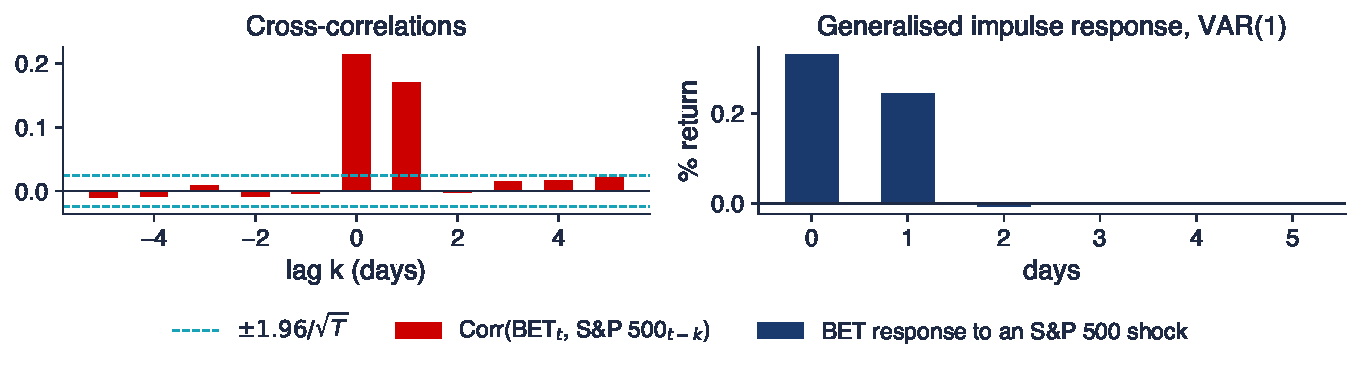
\includegraphics[width=0.96\textwidth,height=0.36\textheight,keepaspectratio]{ch6_sem_b1.pdf}
\end{center}
\vspace{-2mm}
\begin{itemize}
    \item $T = 6\,466$ de zile; CCF: 0{,}21 ($k = 0$), 0{,}170 ($k = 1$), -0{,}003 ($k = -1$); ordine: AIC 9, BIC 1, HQ 1: VAR(1)
    \item S\&P 500 $\to$ BET: $F = 156{,}2$ (p $<$\,0{,}001); BET $\to$ S\&P 500: $F = 2{,}25$ (p 0{,}133); coeficientul lui S\&P$_{t-1}$: 0{,}182 (SE 0{,}015)
    \item Răspunsul generalizat al BET: 0{,}33\% în aceeași zi, 0{,}24\% în ziua următoare, -0{,}007\% după două zile
    \item Interpretare: Wall Street se închide după București, deci știrile din după-amiaza americană ajung la BET abia a doua zi: un efect al fusurilor orare, nu o piață lentă
\end{itemize}\quantlet{TSA\_ch6\_seminar}{\qlurl{TSA_ch6_seminar}}
\end{frame}

\begin{frame}{B2: aceeași întrebare cu randamente săptămînale [Propus]}
\itemsize{\footnotesize}
\begin{itemize}
\item \textbf{Întrebarea}: rezistă precedența S\&P 500 dacă folosim randamente săptămînale, de vineri pînă vineri?
\item \textbf{Date}: randamente logaritmice săptămînale (\%) ale S\&P 500 și BET, din închiderile de vineri; model: B1
\item \textbf{Cerințe}
\begin{enumerate}
    \item Repetați pașii 1--4 din B1 pe randamentele săptămînale.
    \item Comparați corelația încrucișată la decalajul 1 și statistica $F$ cu cele zilnice.
    \item Interpretare: de ce este precedența mult mai slabă la frecvența săptămînală?
\end{enumerate}
\item \textbf{Raportați}: aceleași elemente ca în B1 și două fraze
\item Notebook: secțiunea B2
\end{itemize}
\end{frame}

\ifsolutions
\begin{frame}{B2: rezolvare [Propus]}
\itemsize{\scriptsize}
\begin{center}
\includegraphics[width=0.96\textwidth,height=0.34\textheight,keepaspectratio]{ch6_sem_b2.pdf}
\end{center}
\vspace{-2mm}
\begin{itemize}
    \item $T = 1\,379$ de săptămîni; CCF: 0{,}36 ($k = 0$), 0{,}063 ($k = 1$); ordine: AIC 3, BIC 0, HQ 2: VAR(2)
    \item S\&P 500 $\to$ BET: $F = 4{,}6$ (p 0{,}011), față de $F = 156{,}2$ zilnic; BET $\to$ S\&P 500: p 0{,}914
    \item Interpretare: întîrzierea de o zi cade acum în aceeași săptămînă, deci apare în corelația din aceeași săptămînă (0{,}36), nu la decalaj; rămîne o precedență slabă
\end{itemize}\quantlet{TSA\_ch6\_seminar}{\qlurl{TSA_ch6_seminar}}
\end{frame}
\fi

\begin{frame}{B3: un VAR pentru economia României [Rezolvat]}
\itemsize{\footnotesize}
\begin{itemize}
\item \textbf{Întrebarea}: cum interacționează în România creșterea PIB-ului, inflația și dobînda la 3 luni?
\item \textbf{Date}: $\bY_t = (g_t, \pi_t, i_t)'$, trimestrial, T1 2005--T2 2026
\item \textbf{Cerințe}
\begin{enumerate}
    \item Alegeți $p$ după AIC, BIC și HQ ($p \le 6$) și estimați un VAR(2).
    \item Verificați stabilitatea (cel mai mare modul al valorilor proprii ale matricei companion) și aplicați testul portmanteau cu $h = 8$ și $h = 12$.
    \item Aplicați cele șase teste Granger $F$.
    \item Reprezentați grafic răspunsul ortogonalizat al ROBOR la un șoc al inflației (ordinea $g, \pi, i$) și FEVD pentru ROBOR.
    \item Interpretare: arată rezultatele că banca centrală reacționează la inflație?
\end{enumerate}
\item \textbf{Raportați}: trei ordine, un modul, două teste portmanteau, un tabel cu șase teste, graficul și o frază
\item Notebook: secțiunea B3
\end{itemize}
\end{frame}

\begin{frame}{B3: rezolvare [Rezolvat]}
\itemsize{\scriptsize}
\begin{center}
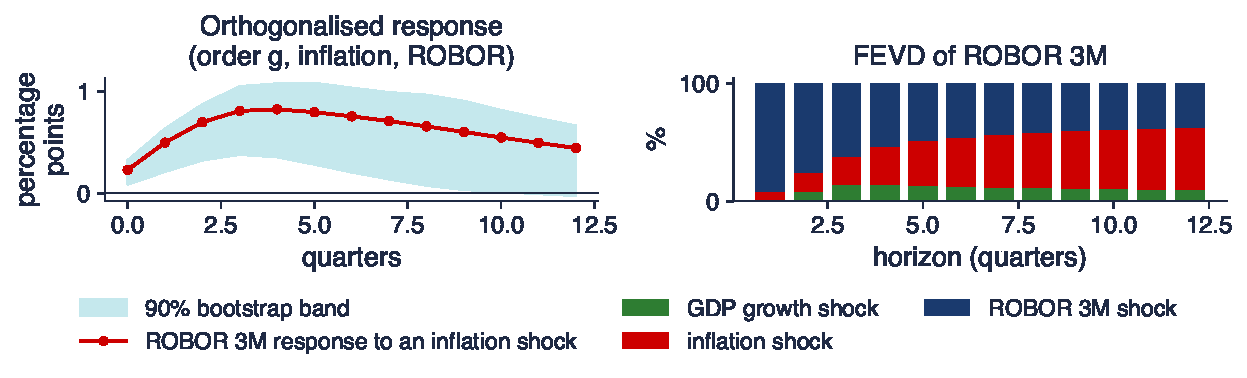
\includegraphics[width=0.96\textwidth,height=0.32\textheight,keepaspectratio]{ch6_sem_b3.pdf}
\end{center}
\vspace{-2mm}
\begin{itemize}
    \item Ordine: AIC 5, BIC 1, HQ 2; VAR(2) pe 84 de trimestre; cel mai mare modul 0{,}869: stabil; $Q_8 = 76{,}7$ (p 0{,}023), $Q_{12} = 105{,}3$ (p 0{,}130)
    \item Granger (p): $g \to i$ 0{,}001, $\pi \to i$ 0{,}011, $i \to g$ 0{,}022, $\pi \to g$ 0{,}059, $i \to \pi$ 0{,}417, $g \to \pi$ 0{,}853
    \item ROBOR după un șoc al inflației: 0{,}23 pp la impact, 0{,}82 pp după 4 trimestre; FEVD pentru ROBOR la 12 trimestre: inflația 53\%, propriile șocuri 37\%
    \item Interpretare: arată că ROBOR \textbf{urmează} inflația, cum ar implica o funcție de reacție; ROBOR este o dobîndă de piață, iar VAR-ul nu poate separa deciziile BNR de așteptările pieței
\end{itemize}\quantlet{TSA\_ch6\_seminar}{\qlurl{TSA_ch6_seminar}}
\end{frame}

\begin{frame}{B4: adăugarea cursului EUR/RON [Propus]}
\itemsize{\footnotesize}
\begin{itemize}
\item \textbf{Întrebarea}: ajută deprecierea leului la prognoza inflației (transmiterea cursului de schimb în prețuri)?
\item \textbf{Date}: $\bY_t = (g_t, s_t, \pi_t, i_t)'$, cu $s_t$ variația trimestrială a cursului EUR/RON, din T4 2005; model: B3
\item \textbf{Cerințe}
\begin{enumerate}
    \item Alegeți $p$ după cele trei criterii ($p \le 4$) și estimați un VAR(2).
    \item Testați dacă $s$ cauzează în sens Granger pe $\pi$, $i$ și $g$ și dacă $i$ și $\pi$ cauzează pe $s$.
    \item Calculați ponderea șocurilor EUR/RON în FEVD pentru inflație la 1, 4, 8 și 12 trimestre.
    \item Interpretare: înseamnă rezultatul că cursul de schimb nu influențează prețurile din România?
\end{enumerate}
\item \textbf{Raportați}: trei ordine, cinci teste $F$, patru ponderi și două fraze
\item Notebook: secțiunea B4
\end{itemize}
\end{frame}

\ifsolutions
\begin{frame}{B4: rezolvare [Propus]}
\itemsize{\scriptsize}
\begin{center}
\includegraphics[width=0.96\textwidth,height=0.32\textheight,keepaspectratio]{ch6_sem_b4.pdf}
\end{center}
\vspace{-2mm}
\begin{itemize}
    \item Ordine: AIC 4, BIC 1, HQ 2; VAR(2) pe 81 de trimestre, cel mai mare modul 0{,}869
    \item $s \to \pi$: $F = 1{,}41$ (p 0{,}252); $s \to i$: p 0{,}281; $s \to g$: p 0{,}012; $i \to s$: p 0{,}035; $\pi \to s$: p 0{,}319
    \item Șocurile EUR/RON explică 0{,}3\%, 0{,}3\%, 0{,}4\% și 0{,}5\% din varianța prognozei inflației; banda răspunsului nu exclude niciodată zero
    \item Interpretare: nu; leul s-a mișcat puțin (curs flotant administrat), mediile trimestriale estompează momentul șocurilor, iar inflația anuală reacționează lent: testul are putere mică, iar lipsa dovezilor nu este o dovadă a lipsei efectului
\end{itemize}\quantlet{TSA\_ch6\_seminar}{\qlurl{TSA_ch6_seminar}}
\end{frame}
\fi


%=============================================================================
\section{Partea C: întrebări deschise și critica unui răspuns AI}
%=============================================================================

\begin{frame}{C1: enigma prețurilor [Propus]}
\itemsize{\footnotesize}
\begin{itemize}
\item \textbf{Întrebarea}: de ce crește inflația după un șoc ROBOR în VAR-ul din B3 și se schimbă acest lucru dacă adăugăm cursul de schimb sau mai multe decalaje?
\item \textbf{Date}: VAR-urile din B3 și B4; ROBOR așezat ultimul; modele: B3, B4
\item \textbf{Cerințe}
\begin{enumerate}
    \item Reprezentați grafic răspunsul inflației la un șoc ROBOR în VAR(2) din B3, în VAR(2) din B4 și într-un VAR(4) cu cele patru variabile din B4.
    \item Raportați cel mai mare și cel mai mic răspuns și orizonturile lor.
    \item Enumerați două informații pe care banca centrală le are, iar VAR-ul nu.
    \item Interpretare: este un răspuns pozitiv al inflației o dovadă că dobînzile mai mari cresc prețurile?
\end{enumerate}
\item \textbf{Raportați}: graficul, șase valori și un plan de proiect
\item Notebook: secțiunea C1
\end{itemize}
\end{frame}

\ifsolutions
\begin{frame}{C1: analiză de referință [Propus]}
\itemsize{\scriptsize}
\begin{center}
\includegraphics[width=0.96\textwidth,height=0.34\textheight,keepaspectratio]{ch6_sem_c1.pdf}
\end{center}
\vspace{-2mm}
\begin{itemize}
    \item Răspunsul maxim: 0{,}16 pp după 2 trimestre (B3); 0{,}15 pp după 3 (B4); 0{,}16 pp după 1 (VAR(4)), apoi -0{,}07 pp după 4
    \item Banca vede așteptările inflaționiste, prognozele prețurilor la energie și alimente, datele despre salarii și planurile fiscale; cînd crește dobînda pentru că anticipează inflația, VAR-ul numește mișcarea „șoc” urmat de inflație
    \item Interpretare: nu; semnalează un șoc identificat greșit (informație omisă), enigma prețurilor din \refSimsPP
    \item Proiect: adăugați un indice al prețurilor materiilor prime, dobînda din zona euro sau așteptările din anchete și comparați răspunsurile
\end{itemize}\quantlet{TSA\_ch6\_seminar}{\qlurl{TSA_ch6_seminar}}
\end{frame}
\fi

\begin{frame}{C2: verificați un răspuns AI [Propus]}
\itemsize{\scriptsize}
\begin{itemize}
    \item Un student a cerut unui asistent AI să analizeze VAR-ul din B3. Răspunsul:
    \item \aiprompt{(a) AIC alege p = 5, deci ordinul adevărat al economiei este 5.}
    \item \aiprompt{(b) Cel mai mare modul al valorilor proprii ale lui A1 este 1{,}37, deci VAR(2) este exploziv.}
    \item \aiprompt{(c) Testul portmanteau la 8 decalaje are p = 0{,}023, deci reziduurile sînt zgomot alb.}
    \item \aiprompt{(d) Creșterea PIB-ului cauzează ROBOR în sens Granger, deci creșterea mai rapidă determină BNR să crească dobînzile.}
    \item \aiprompt{(e) Răspunsurile la impuls Cholesky nu depind de ordinea variabilelor.}
    \item \aiprompt{(f) Pe fiecare rînd al FEVD ponderile însumează 100\%.}
    \item Cerințe
    \begin{itemize}
        \item 1. Pentru fiecare afirmație, precizați dacă este corectă; dacă nu este, formulați afirmația corectă și, acolo unde se poate, dați valoarea corectă din notebook (secțiunea C2).
        \item 2. Raportați: o listă de șase verdicte, fiecare cu un rînd de justificare.
    \end{itemize}
\end{itemize}
\end{frame}

\ifsolutions
\begin{frame}{C2: rezolvare [Propus]}
\itemsize{\scriptsize}
\begin{itemize}
    \item (a) Greșit: criteriile aleg un model pentru un eșantion; BIC alege 1, HQ 2; nu există un ordin „adevărat” de descoperit
    \item (b) Greșit: stabilitatea unui VAR(2) se decide pe matricea companion; cel mai mare modul al ei este 0{,}87 $< 1$: stabil
    \item (c) Greșit: p = 0{,}023 $< 0{,}05$ respinge zgomotul alb la 8 decalaje (la 12 decalaje nu se respinge)
    \item (d) Greșit: cauzalitatea Granger înseamnă predictibilitate; ROBOR este o dobîndă de piață și ambele pot reacționa la un al treilea factor
    \item (e) Greșit: ordinea decide ce variabilă reacționează la impact (A3, B3)
    \item (f) Corect
\end{itemize}\quantlet{TSA\_ch6\_seminar}{\qlurl{TSA_ch6_seminar}}
\end{frame}
\fi


%=============================================================================
\section{Încheiere}
%=============================================================================

\begin{frame}{Idei de reținut}
\itemsize{\small}
\begin{itemize}
    \item Stabilitatea: valorile proprii ale lui $\bA$ (sau ale matricei companion) în interiorul cercului unitate; atunci prognozele converg spre $\boldsymbol{\mu}$
    \item Testul Granger $F$: comparăm ecuația cu și fără decalajele variabilei candidate
    \item Răspunsurile Cholesky depind de ordine; cele generalizate nu
    \item S\&P 500 precedă BET cu o zi din cauza fusurilor orare; ROBOR urmează inflația din România
    \item Un răspuns AI este o ciornă: verificați sensul fiecărei afirmații și ce matrice decide stabilitatea
\end{itemize}
\end{frame}

\begin{frame}{După seminar}
\itemsize{\small}
\begin{itemize}
    \item Cursul 6 dezvoltă fiecare temă de azi: procese vectoriale, forma companion, alegerea numărului de decalaje, diagnosticarea, cauzalitatea Granger și capcanele ei, răspunsurile la impuls, FEVD, spillover-ul, prognoza, VAR-urile structurale
    \item Încercați cerințele [Propus] în notebook
    \item C1 poate deveni un proiect de echipă: șocurile de politică monetară din România într-un VAR extins
    \item Lectură: \refHP, cap.~7; \refFPP, secț.~12.3; \refSW
    \item \textbf{Seminarul are rol de exercițiu și nu se notează; rezolvările cerințelor [Propus] se discută la seminar}
\end{itemize}
\end{frame}


%=============================================================================
\section{Bibliografie}
%=============================================================================

\begin{frame}{Bibliografie}
\itemsize{\tiny}
\begin{itemize}
    \item Granger, C. W. J. (1969). Investigating causal relations by econometric models and cross-spectral methods. \textit{Econometrica}, 37(3), 424--438. \href{https://doi.org/10.2307/1912791}{doi:10.2307/1912791}
    \item Huang, C., \& Petukhina, A. (2022). \textit{Applied Time Series Analysis and Forecasting with Python}. Springer. \href{https://doi.org/10.1007/978-3-031-13584-2}{doi:10.1007/978-3-031-13584-2}
    \item Hyndman, R. J., \& Athanasopoulos, G. (2021). \textit{Forecasting: Principles and Practice} (3rd ed.), Section 12.3, Vector autoregressions. OTexts. \href{https://otexts.com/fpp3/VAR.html}{otexts.com/fpp3/VAR.html}
    \item Lütkepohl, H. (2005). \textit{New Introduction to Multiple Time Series Analysis}. Springer. \href{https://doi.org/10.1007/978-3-540-27752-1}{doi:10.1007/978-3-540-27752-1}
    \item Pesaran, M. H., \& Shin, Y. (1998). Generalized impulse response analysis in linear multivariate models. \textit{Economics Letters}, 58(1), 17--29. \href{https://doi.org/10.1016/S0165-1765(97)00214-0}{doi:10.1016/S0165-1765(97)00214-0}
    \item Sims, C. A. (1980). Macroeconomics and reality. \textit{Econometrica}, 48(1), 1--48. \href{https://doi.org/10.2307/1912017}{doi:10.2307/1912017}
    \item Sims, C. A. (1992). Interpreting the macroeconomic time series facts: The effects of monetary policy. \textit{European Economic Review}, 36(5), 975--1000. \href{https://doi.org/10.1016/0014-2921(92)90041-T}{doi:10.1016/0014-2921(92)90041-T}
    \item Stock, J. H., \& Watson, M. W. (2001). Vector autoregressions. \textit{Journal of Economic Perspectives}, 15(4), 101--115. \href{https://doi.org/10.1257/jep.15.4.101}{doi:10.1257/jep.15.4.101}
\end{itemize}
\end{frame}

\end{document}
